\section{ドップラー効果と衝撃波}

% ===========================================================================
%  再編（2026-09-05）：第2章 波動 の第17回．
%  原本の 第23回「ドップラー効果(1)」の全体（23.1〜23.6）と，第24回の 24.1 斜めドップラー効果・
%  24.2 斜めドップラー効果の式の導出問題・24.3 衝撃波 を合わせて1回とした．
%  （第24回の残り 24.3 光速度／24.4 光の屈折／24.5 ホイヘンスの原理は第18回の冒頭へ移してある）
%  ・練習は 原本 第23回［30］〜［40］の11題 ＋ 第24回のドップラー系4題［42］［43］［48］［49］．
%    A問題の［30］［31］（ともに「基本事項の確認」）を1題に統合したので 14題．設問は1つも落として
%    いない（［30］の(1)(2)(3)＋［31］の(1)(2) がそのまま新［29］の(1)〜(5) になっている）。
%  ・問題番号は第16回の［21］〜［28］に続けて［29］〜［42］（\setcounter{qno}{28}）．
%    新旧対応：［29］＝㉓[30]+[31]／［30］＝㉓[32]／［31］＝㉓[33]／［32］＝㉓[34]／
%    ［33］＝㉓[35]／［34］＝㉓[36]／［35］＝㉓[37]／［36］＝㉓[38]／［37］＝㉔[42]／
%    ［38］＝㉔[43]／［39］＝㉓[39]／［40］＝㉓[40]／［41］＝㉔[48]／［42］＝㉔[49]．
%  ・原本の例題7題（13〜19）をそのまま採用した（削除なし）。挿入位置も原本と同じ．
%      例題13〈波源が媒質に対して動く場合の効果〉      … 17.2 の後（原本 p107）
%      例題14〈観測者が媒質に対して動く場合の効果〉    … 17.3 の後（原本 p108）
%      例題15〈関係式による振動数の直接計算〉          … 17.4 の後（原本 p110）
%      例題16〈風がある場合のドップラー効果〉          … 17.5 の後（原本 p111）
%      例題17〈反射波によるドップラー効果〉            … 17.6 の後（原本 p112）
%      例題18〈斜めドップラー効果〉                    … 17.7 の後（原本 p113）
%      例題19〈斜めドップラー効果の導出〉              … 17.8 の後（原本 p114）
%    原本は「問題枠 →（指針）＝空欄 →【KEY】」で解答が載っていないため，
%    【指針】と【解答】は書き起こした（KEY と問題文・図は原本からの転写）。
%    例題15の図は例題13の図と同一（原本でも同じ4配置を再掲）なので同じ png を使っている．
%  ・旧 physics_ch24.tex には原本の 24.2「斜めドップラー効果の式の導出問題」の節が落ちていた
%    （例題19が入る節）。原本 p114 から復活させた．
%  ・{\bf …} は新スタイルに合わせて {\gtfamily …} に置き換え，単位は \U{} に統一．
%    旧レイアウト用の \vspace や figure 環境は全て取り除き，wrapfigure の [N] は図の実高
%    （.xbb から算出）に合わせて付け直して \bsNeed を入れた．
%  ・図は texify_draft/mkfig_new17.py＋jobs_new17.py（問題編からの切り出し35枚）／
%    mkfig_new17ex.py（原本 20161215143926.pdf の p107・p111・p112・p113・p114 から5枚）で
%    再生成できる．
% ===========================================================================

% 例題番号：波動（原本 第3章）の例題は章の先頭から通し番号．第16回で10〜12を使った．
\setcounter{nombre}{12}

\subsection{ドップラー効果を考えるための基礎知識}

波源，もしくは観測者が動くときには，波源が本来出している振動数とは異なる振動数の波が観測される．
この現象を{\gtfamily ドップラー効果}という．
波源が動くか，観測者が動くかによって起こる現象および観測される振動数は異なる．
この現象を，まずは一直線上で波源と観測者が運動する場合について考える．

ドップラー効果を考えていくために必要となる基礎知識をまとめておく．

\begin{matome}{ドップラー効果を考えるための基礎知識}
\begin{description}
\item[\MARU{1}] 振動数とは，単位時間あたりにやりとりする波の数のことである．すなわち，\\
\hspace{3mm}{\gtfamily 波源の振動数\hspace{18mm}＝\hspace{2mm}波源が単位時間あたりに出す波の数}\\
\hspace{3mm}{\gtfamily 観測者が受け取る振動数\hspace{2mm}＝\hspace{2mm}観測者が単位時間あたりに受け取る波の数}
\item[\MARU{2}] 波長とは，$\sin$カーブひとつ分の長さ（＝山−山の間隔）のことである．
\item[\MARU{3}] 空間中を伝わる波が固有に持っているのは，{\gtfamily 波の伝わる速度と波の波長である．}振動数は\MARU{1}の通り「単位時間あたりに何個の波をやりとりするか」であるから，{\gtfamily 波源・観測者がどう動くかによって値が変わる．}（媒質に対して静止した観測者が数える振動数だけは$\dfrac{c}{\lambda}$に定まる．）
\item[\MARU{4}] いかなる場合でも，{\gtfamily 波の伝わる速度は媒質に対して不変である．観測者，波源が動いたとしても媒質中を伝わる波の速度は変わらない．}ただし，媒質が動くとき（音の場合は風があるとき）は媒質そのものが移動するため，地面に対する波の速度は変化する．
\end{description}
\end{matome}

これらの知識を利用して，波源や観測者が動いた場合に空間中を伝わる波がどのように変化するのか考えていく．

\bsNeed{83mm}
\subsection{波源が媒質に対して動く場合}
\begin{wrapfigure}[16]{r}[5mm]{100mm}
  \centering
  \vspace{-5mm}
  
\includegraphics[keepaspectratio,width=100mm]
  {text_p106_fig1.png}
\end{wrapfigure}
振動数$f\U{Hz}$の波源が図のように右向きに速度$v\U{m/s}$で進んでいる場合について考える．
このときの波の速さを$c\U{m/s}$とし，$v<c$であるとする．

今，時刻$t=0\U{s}$に波源が$\mathrm{A}$点にいたとすると，時刻$t=0\U{s}$に$\mathrm{A}$点から出た波は，$\Delta t\U{s}$後には$\mathrm{A}$点から左右両方向に$c\Delta t\U{m}$だけ進んでいる．
一方，波源自身はこの$\Delta t\U{s}$の間に距離$v\Delta t\U{m}$だけ右方向へ移動して$\mathrm{B}$点に達している．

この$\Delta t\U{s}$の間に波源は左右両方向に$f\Delta t$個の波を出しているわけなので，波源の進行方向には距離$c\Delta t-v\Delta t\U{m}$の区間に$f\Delta t$個の波が，また波源の進行の逆方向には距離$c\Delta t+v\Delta t\U{m}$の区間に$f\Delta t$個の波が存在していることになる．
波ひとつあたりの長さが波長であるから，
\[\text{波の進行方向に出た波の波長}\hspace{6mm}\lambda_1=\frac{c\Delta t-v\Delta t}{f\Delta t}=\frac{c-v}{f}\U{m}\]
\[\text{その逆方向に出た波の波長}\hspace{8mm}\lambda_2=\frac{c\Delta t+v\Delta t}{f\Delta t}=\frac{c+v}{f}\U{m}\]
となっていることがわかる．
静止している波源から出てくる場合の波長は$\lambda=\dfrac{c}{f}\U{m}$であるから，{\gtfamily 波源の進行方向では空間を伝わる波は圧縮されて波長が短くなり，その逆方向では波は伸ばされて波長が長くなる}ことが言える．

\begin{matome}{動く波源から出る波}
\hspace{3mm} 波源が媒質に対して動くときの効果 ＝ 空間（媒質）を伝わる波の波長が変化する\\
\hspace{10mm} 波の進行方向\hspace{5mm}波長が$\lambda_1=\dfrac{c-v}{f}\U{m}$に圧縮\\
\hspace{10mm} その逆方向\hspace{8mm}波長が$\lambda_2=\dfrac{c+v}{f}\U{m}$に伸長\\
\hspace{3mm} 波の速さは$c\U{m/s}$のまま不変
\end{matome}

\bsNeed{100mm}
%%%%%  例題13（17.2 のまとめ枠の直後）＝ 原本【例題13】〈波源が媒質に対して動く場合の効果〉（p107）  %%%%%%
% 問題文・図・KEY は原本からの転写。原本には解答が載っていないので【指針】【解答】は書き起こした。
\begin{reidaiunit}
\begin{reidai}{波源が媒質に対して動く場合の効果}
\hspace{1zw}振動数$f\U{Hz}$の音源がある．音源と観測者が次の各図のように移動する場合それぞれについて，音源から観測者の方向に向かって空間中を伝わっている音波の速度$c^\prime\U{m/s}$および波長$\lambda^\prime\U{m}$を求めよ．ただし，この温度における音速を$c\U{m/s}$とし，$u,v<c$であるとする．
\begin{center}
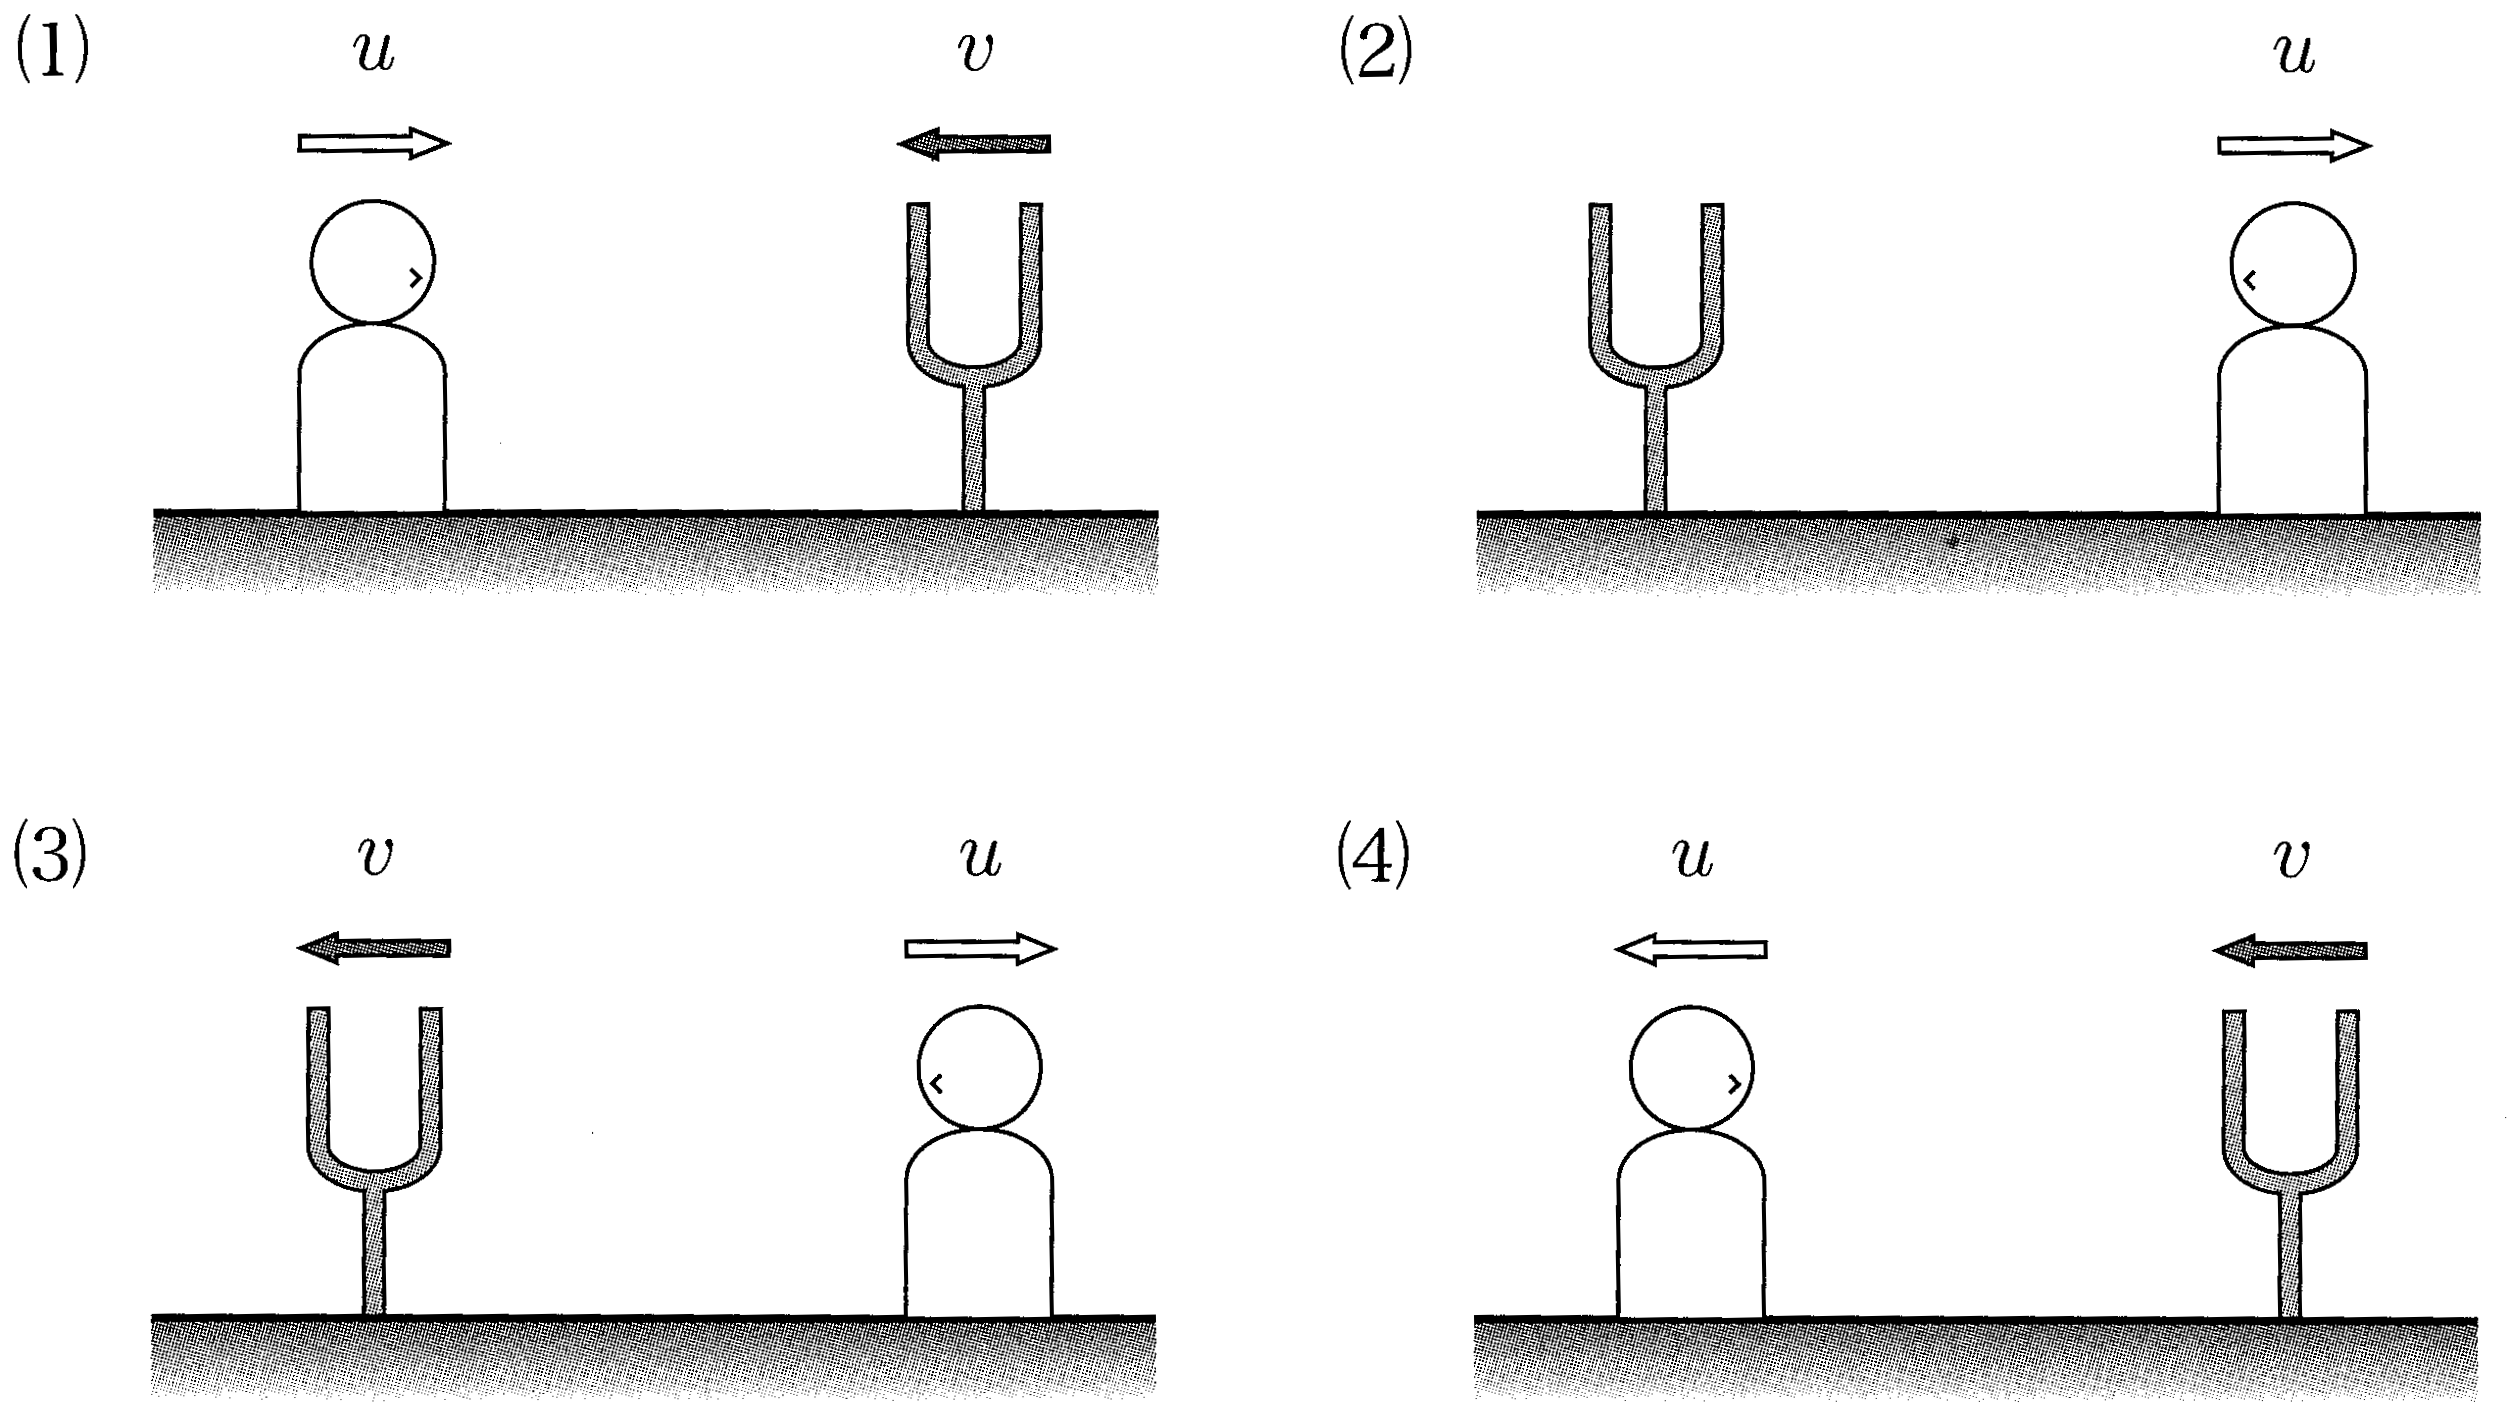
\includegraphics[keepaspectratio,width=115mm]{fig/n17_ex13_z.png}
\end{center}
\end{reidai}

\begin{sisinE}
関係式を当てはめようとする考え方だとミスを犯しやすい．$\Delta t$秒後の波の状態を描いて，ひとつあたりの波の幅を計算するという考え方を適用すれば，式を暗記しなくても波長を求められる．

{\gtfamily 波長を変えるのは波源の運動だけであって，観測者がどう動いても空間を伝わる波の波長・速度は変わらない．}また風がないので，波の速度はどの場合も$c\U{m/s}$である．
まず{\gtfamily 音源から観測者へ向かう向き}（＝考えている音波の進行方向）を決め，その向きを正として波源の速度成分を読み取ればよい．
\end{sisinE}
\Key{波の波長 ＝ 波ひとつあたりの長さ\quad 波は出された点を中心として速さ$c\U{m/s}$で広がっていく}

\begin{kaitou}
\hspace{1zw}いずれの場合も媒質（空気）は静止しているので，空間を伝わる音波の速度は
\Ana{c^\prime=c\U{m/s}\Ans}
である．波長は波源の運動だけで決まるので，音源から観測者へ向かう向きを正として音源の速度成分を読み取る．
\begin{komon}
\ko{1} 音源は右側にあり，音は左向きに進む．音源の速度$v$は左向き，すなわち音の進行方向と同じ向きなので波長は圧縮されて，
       \Ana{\lambda^\prime=\frac{c-v}{f}\U{m}\Ans}
\ko{2} 音源は静止しているので波長は変化せず，
       \Ana{\lambda^\prime=\frac{c}{f}\U{m}\Ans}
\ko{3} 音源は左側にあり，音は右向きに進む．音源の速度$v$は左向き，すなわち音の進行方向と逆向きなので波長は伸長されて，
       \Ana{\lambda^\prime=\frac{c+v}{f}\U{m}\Ans}
\ko{4} 音源は右側にあり，音は左向きに進む．音源の速度$v$は左向き，すなわち音の進行方向と同じ向きなので波長は圧縮されて，
       \Ana{\lambda^\prime=\frac{c-v}{f}\U{m}\Ans}
\end{komon}
\end{kaitou}
\begin{chuu}
(1)と(4)は観測者の運動が違うだけで音源の運動は同じであり，空間を伝わる波の様子はまったく同じである．観測者の運動は次節で見るように「受け取る振動数」だけを変える．
\end{chuu}
\end{reidaiunit}

\bsNeed{97mm}
\subsection{観測者が媒質に対して動く場合}
\begin{wrapfigure}[19]{r}[5mm]{100mm}
  \centering
  \vspace{-5mm}
  
\includegraphics[keepaspectratio,width=100mm]
  {text_p108_fig1.png}
\end{wrapfigure}
空間中を，波長$\lambda\U{m}$の波が速さ$c\U{m/s}$で伝わってくるとき，これを波の伝わる方向と同じ向きに速さ$u\U{m/s}\ (u<c)$で動いている観測者が受け取るときに観測する振動数を求める．

今，時刻$t=0\U{s}$にちょうど$\mathrm{A}$点にて観測者と重なった波は，$\Delta t\U{s}$後には距離$c\Delta t\U{m}$だけ進んで$\mathrm{D}$点に達する．
一方，観測者はこの$\Delta t\U{s}$の間に距離$u\Delta t\U{m}$だけ進んだ$\mathrm{B}$点にいる．

この$\Delta t\U{s}$の間に{\gtfamily 観測者は自分自身を通過していった（追い越していった）波を受け取っている．}
観測者を追い越していったのは$\mathrm{B}$から$\mathrm{D}$の区間にある波，すなわち距離$c\Delta t-u\Delta t\U{m}$の区間に存在する波である．
よって，観測者が聞く振動数，つまり$1\U{s}$あたりに受け取る波の個数$f^\prime\U{Hz}$は
\[f^\prime\Delta t=\frac{c\Delta t-u\Delta t}{\lambda}\hspace{5mm}\Leftrightarrow\hspace{5mm}f^\prime=\frac{c-u}{\lambda}\U{Hz}\]
で与えられる．

{\gtfamily 観測者が動いていても，空間（媒質）を伝わる波の波長・速度は不変であることに注意せよ．}
観測者が動く場合は，観測される振動数のみが変化するため，$c=f^\prime\lambda$の式を立てて観測者の聞く振動数を求めることはできない．

\begin{matome}{観測者が動く場合}
\hspace{3mm} 観測者が媒質に対して動くときの効果\\
\hspace{10mm} $\Rightarrow$\hspace{2mm}観測される振動数のみ変化，他のすべての物理量は変化せず\\
\hspace{3mm} 観測者の速度を$u\U{m/s}$（波の進行方向と同じ向きを正）とすると，\\
\hspace{10mm} 観測者が聞く振動数\hspace{5mm}$f^\prime=\dfrac{c-u}{\lambda}\U{Hz}$
\end{matome}

\bsNeed{80mm}
%%%%%  例題14（17.3 のまとめ枠の直後）＝ 原本【例題14】〈観測者が媒質に対して動く場合の効果〉（p108）  %%%%%%
\begin{reidaiunit}
\begin{reidai}{観測者が媒質に対して動く場合の効果}
\hspace{1zw}例題13の各場合について，観測者が聞く振動数$f^\prime\U{Hz}$を，$c,\lambda^\prime,u$を用いて表せ．
\end{reidai}

\begin{sisinE}
観測者が聞く振動数とは{\gtfamily 単位時間あたりに観測者が受け取る波の数}である．
波長$\lambda^\prime\U{m}$の波が速さ$c\U{m/s}$で伝わってくる空間を観測者が動くとき，$1\U{s}$の間に観測者を追い越していく波は，長さ$c-u^\prime\U{m}$の区間にある波である（$u^\prime$は{\gtfamily 波の進行方向を正としたときの観測者の速度}）．
したがって
\[f^\prime=\frac{c-u^\prime}{\lambda^\prime}\U{Hz}\]
となる．例題13と同じく，まず音の進行方向（音源から観測者へ向かう向き）を正に決めてから，観測者の速度の符号を読み取ること．
\end{sisinE}
\Key{観測者が聞く振動数\quad $\Rightarrow$\quad 単位時間あたりに受け取る波の数を数える}

\begin{kaitou}
\begin{komon}
\ko{1} 音は左向きに進み，観測者の速度$u$は右向き（音の進行方向と逆向き）である．観測者は波に向かっていくので，
       \Ana{f^\prime=\frac{c+u}{\lambda^\prime}\U{Hz}\Ans}
\ko{2} 音は右向きに進み，観測者の速度$u$も右向き（音の進行方向と同じ向き）である．観測者は波から逃げるので，
       \Ana{f^\prime=\frac{c-u}{\lambda^\prime}\U{Hz}\Ans}
\ko{3} 音は右向きに進み，観測者の速度$u$も右向きであるから，(2)と同じく
       \Ana{f^\prime=\frac{c-u}{\lambda^\prime}\U{Hz}\Ans}
\ko{4} 音は左向きに進み，観測者の速度$u$も左向き（音の進行方向と同じ向き）であるから，
       \Ana{f^\prime=\frac{c-u}{\lambda^\prime}\U{Hz}\Ans}
\end{komon}
\end{kaitou}
\begin{chuu}
例題13の$\lambda^\prime$を代入すれば，各場合の$f^\prime$が$c,u,v,f$で書ける．たとえば(1)なら
\[f^\prime=\frac{c+u}{\lambda^\prime}=\frac{c+u}{c-v}f\U{Hz}\]
となる．これが次節で述べるドップラー効果の関係式にほかならない．
\end{chuu}
\end{reidaiunit}

\subsection{波源・観測者の両方が媒質に対して動く場合}

以上の考え方，すなわち，
\begin{description}
\item[\MARU{1}] まず空間中を伝わる波の波長$\lambda^\prime\U{m}$を求める．
\item[\MARU{2}] 観測者が単位時間あたりに受け取る波の数を数える．
\end{description}
という2段階を踏めば，波源・観測者の両方が動く場合も含めたすべての場合について観測者が聞く振動数を求めることが原理的に可能である．
しかしこれは2段階を踏むため計算が面倒であること，また波長については問われず振動数のみが問われることが多いため，この2段階を合体させて途中の$\lambda^\prime$を求める過程を省いたものが，ここで述べるドップラー効果の関係式である．

\begin{zuright}{50mm}
\hspace{1zw}観測者と波源が右図のような位置関係で，各々が図のような速度で動いている場合，波源の振動数を$f\U{Hz}$とすれば，波源から観測者に向かって空間を伝わる波長$\lambda^\prime\U{m}$は
\[\lambda^\prime=\frac{c-v}{f}\U{m}\]
である．これを観測者が受け取ったときの振動数$f^\prime\U{Hz}$は
\[f^\prime=\frac{c-u}{\lambda^\prime}\U{Hz}\]
であり，上の式を代入して整理すると，
\[f^\prime=\frac{c-u}{c-v}f\U{Hz}\]
となる．
\zusep

\includegraphics[keepaspectratio,width=50mm]{text_p109_fig1.png}
\end{zuright}
しかしこの式は観測者と波源の左右関係および速度ベクトルの向きによって，見かけ上さまざまに変化する．
そこで次のようにして立てるとよい．

\begin{matome}{ドップラー効果の関係式}
\begin{description}
\item[\MARU{1}] 波の進行方向を速度の正の方向とする．
\item[\MARU{2}] 分数部分は波源の上に観測者が乗る形で，
\[\text{観測される振動数}=\frac{\text{波の速さ}-\text{観測者の速度}}{\text{波の速さ}-\text{波源の速度}}\times\text{波源の振動数}\]
として振動数を求める．
\end{description}
\end{matome}

ただし，この式を用いて計算した振動数$f^\prime\U{Hz}$はあくまで観測者が聞く振動数であって，空間を伝わる波そのものが持っている振動数ではない．

また，この関係式からでは空間を伝わる波の波長$\lambda^\prime\U{m}$を求めることはできない．
$\lambda^\prime\U{m}$を求めたい場合は，波源が動く場合の波長の変化を原理に立ち戻って求めよ．

\bsNeed{100mm}
%%%%%  例題15（17.4 のまとめ枠の直後）＝ 原本【例題15】〈関係式による振動数の直接計算〉（p110）  %%%%%%
% 図は例題13と同一（原本でも同じ4配置を再掲している）ので同じ png を使う。
\begin{reidaiunit}
\begin{reidai}{ドップラー効果の関係式による振動数の直接計算}
\hspace{1zw}振動数$f\U{Hz}$の音源がある．音源と観測者が次の各図のように移動する場合それぞれについて，観測者が観測する音の振動数$f^\prime\U{Hz}$を求めよ．ただし，この温度における音速を$c\U{m/s}$とし，速さ$u\U{m/s}$, $v\U{m/s}$は$u,v<c$を満たすとする．
\begin{center}
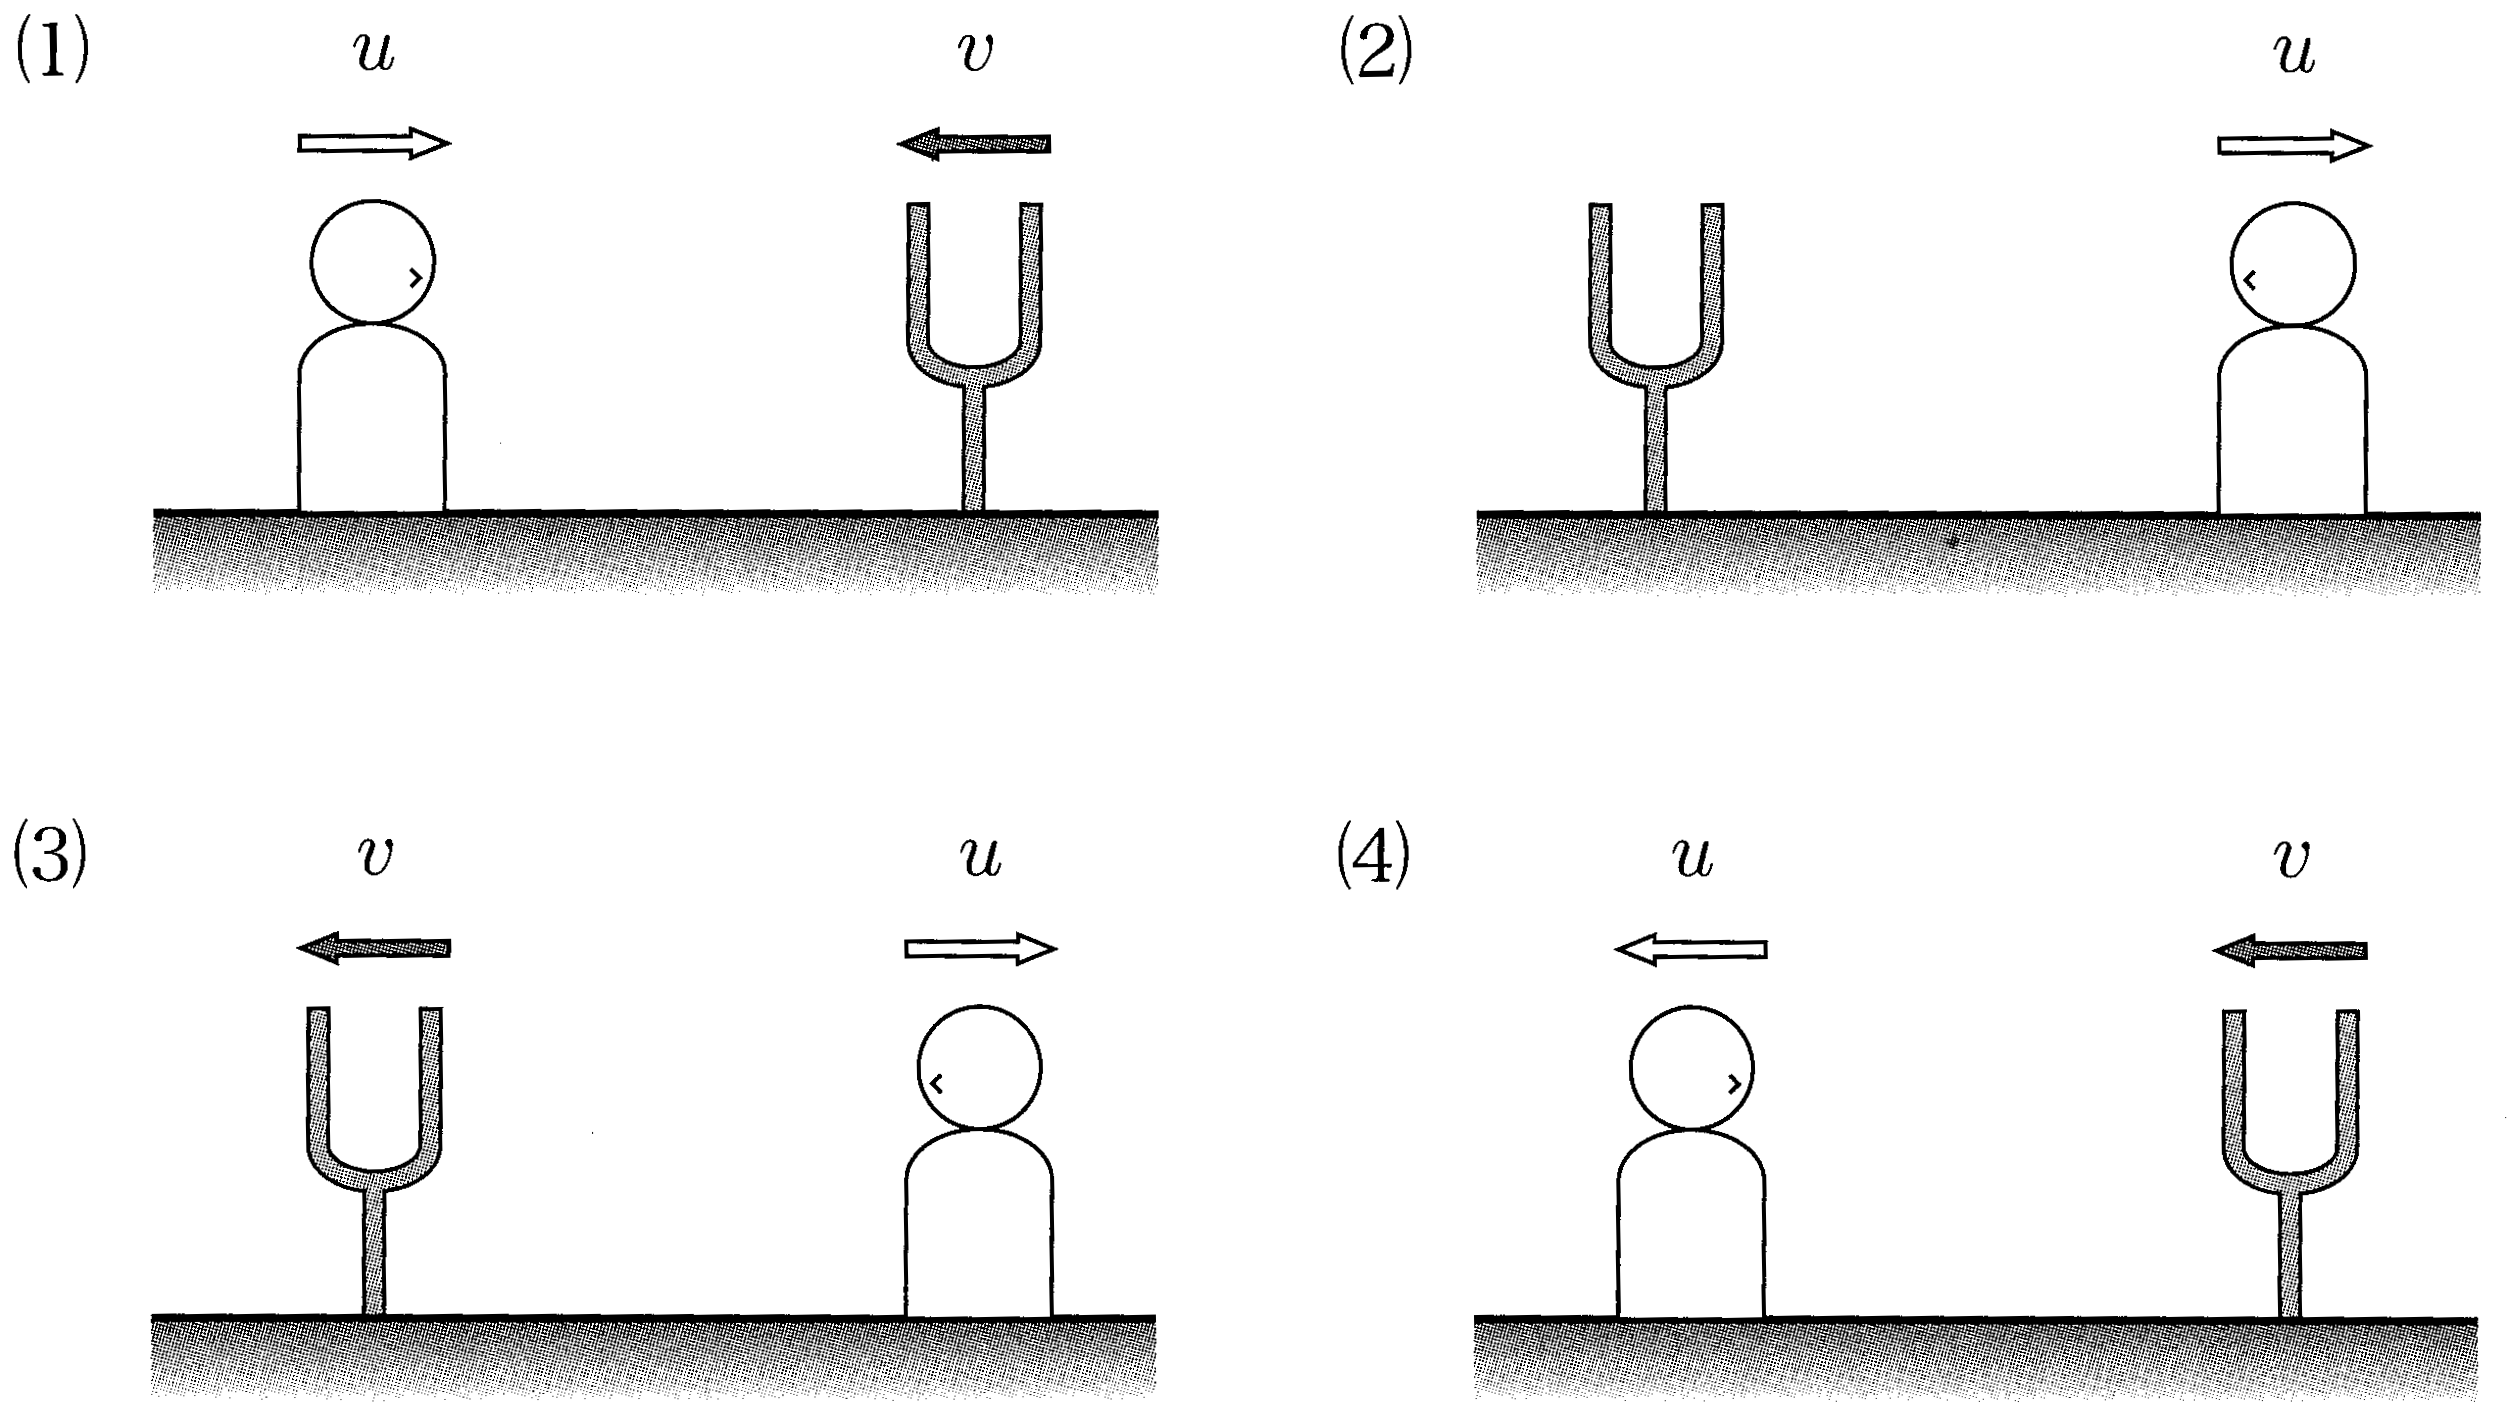
\includegraphics[keepaspectratio,width=115mm]{fig/n17_ex13_z.png}
\end{center}
\end{reidai}

\begin{sisinE}
例題13・14を2段階に分けずに，関係式で一気に計算する練習である．
{\gtfamily 波の進行方向（音源から観測者へ向かう向き）を正}に取り，観測者・波源の速度をその向きの成分として符号つきで代入する．
分子が観測者，分母が波源であることを間違えないこと（{\gtfamily 波源の上に観測者が乗る}形で覚えるとよい）．
\end{sisinE}
\Key{\MARU{1} 波の進行方向を速度の正の方向とする\quad
     \MARU{2} $f^\prime=\dfrac{\text{波の速さ}-\text{観測者の速度}}{\text{波の速さ}-\text{波源の速度}}\times f$}

\begin{kaitou}
\begin{komon}
\ko{1} 音は左向きに進むので左向きを正とする．観測者の速度は$-u$，波源の速度は$+v$であるから，
       \Ana{f^\prime=\frac{c-(-u)}{c-v}f=\frac{c+u}{c-v}f\U{Hz}\Ans}
\ko{2} 音は右向きに進むので右向きを正とする．観測者の速度は$+u$，波源は静止しているから，
       \Ana{f^\prime=\frac{c-u}{c}f\U{Hz}\Ans}
\ko{3} 音は右向きに進むので右向きを正とする．観測者の速度は$+u$，波源の速度は$-v$であるから，
       \Ana{f^\prime=\frac{c-u}{c+v}f\U{Hz}\Ans}
\ko{4} 音は左向きに進むので左向きを正とする．観測者の速度は$+u$，波源の速度は$+v$であるから，
       \Ana{f^\prime=\frac{c-u}{c-v}f\U{Hz}\Ans}
\end{komon}
\end{kaitou}
\begin{chuu}
例題13で求めた$\lambda^\prime$を例題14の式に代入した結果と一致することを確かめよ．
関係式は2段階の考え方を合体させただけのものであって，新しい物理が入っているわけではない．
\end{chuu}
\end{reidaiunit}

\subsection{風がある場合のドップラー効果}

ドップラー効果は媒質に対する波源・観測者の移動が原因となって起こるため，本質的には媒質の立場に立ち，それに対する波源・観測者の相対速度を利用してドップラー効果の式を立てる必要がある．
しかし，地面を基準にとって考えて，波を伝える媒質そのものが動くことにより波が加速されたり減速されたりすると考えればよい．

音の場合，波を伝える媒質は空気なので，風が吹いている場合はその風速の分だけ媒質が地面に対して速度をもって移動していると考えればよい．
結果，地面から見た場合は音速が風速の分だけ増減したものとしてドップラー効果の関係式に代入すればよい．

\begin{matome}{風がある場合の音波の速さ}
\hspace{3mm} 音速を$c\U{m/s}$，風速を$w\U{m/s}$とするとき，\\
\hspace{5mm} ・風下側に音波が伝わるとき\hspace{2mm}$\Rightarrow$\hspace{2mm}音波は風に押されて$c+w\U{m/s}$に加速される\\
\hspace{5mm} ・風上側に音波が伝わるとき\hspace{2mm}$\Rightarrow$\hspace{2mm}音波は風に押し戻されて$c-w\U{m/s}$に減速される
\end{matome}

\bsNeed{95mm}
%%%%%  例題16（17.5 のまとめ枠の直後）＝ 原本【例題16】〈風がある場合のドップラー効果〉（p111）  %%%%%%
\begin{reidaiunit}
\begin{reidai}{風がある場合のドップラー効果}
\hspace{1zw}振動数$f\U{Hz}$の音を出す音源がある．風のないとき，音源から観測者に向かう音波の，地面に対する速さ$c\U{m/s}$とする．図のように風速$w\U{m/s}$の風が吹いており，音源・観測者が動く場合について，音源から観測者に向かう音波の，地面に対する速さ$c^\prime\U{m/s}$を求め，それをもとに観測者が聞く振動数$f^\prime\U{Hz}$を求めよ．また，空間中を伝わっている波の波長$\lambda^\prime\U{m}$を求めよ．
\begin{center}
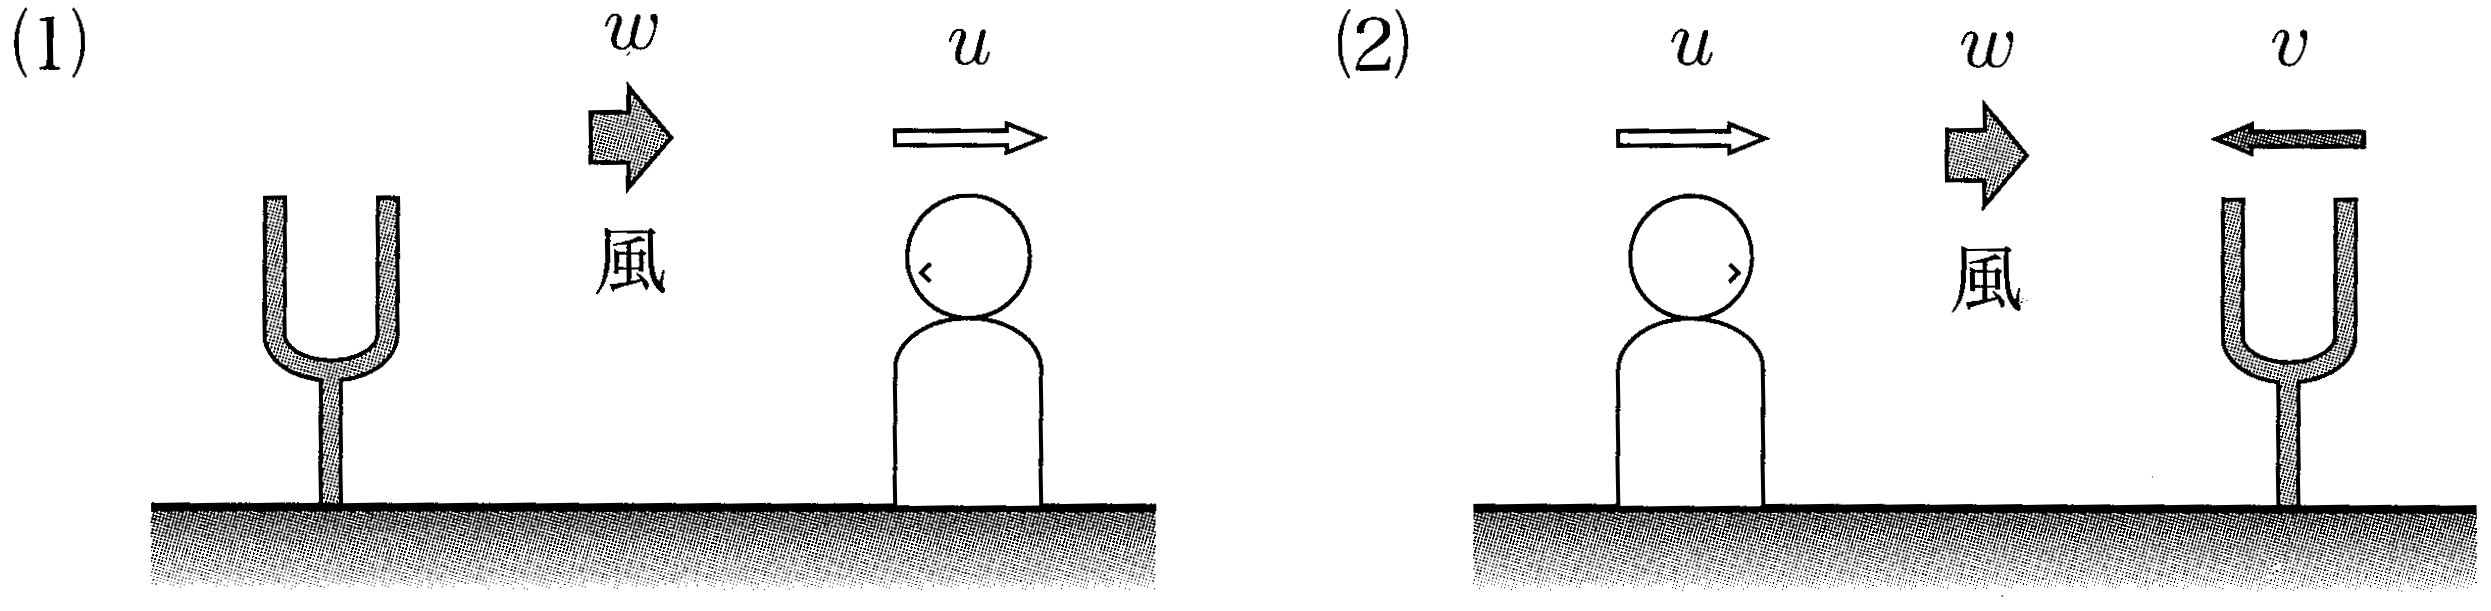
\includegraphics[keepaspectratio,width=110mm]{fig/n17_ex16_z.png}
\end{center}
\end{reidai}

\begin{sisinE}
風があるときは{\gtfamily 地面に対する音速が$c\pm w$に変わっただけ}と考えて，あとは今までどおりに扱えばよい．
音の進行方向と風向きが同じなら追い風で$c+w$，逆なら向かい風で$c-w$である．

波長は「$1\U{s}$あたりに波源が出した$f$個の波が，どれだけの長さの区間に並ぶか」で決まるから，
\[\lambda^\prime=\frac{(\text{地面に対する音速})-(\text{波源の速度})}{f}\]
となる（いずれも音の進行方向を正とした値）．
\end{sisinE}
\Key{風がある場合\quad $\Rightarrow$\quad 地面に対する音速を$c\pm w$に置き換えるだけ}

\begin{kaitou}
\begin{komon}
\ko{1} 音は音源（左）から観測者（右）へ，すなわち右向きに進む．風も右向きなので追い風であり，
       \Ana{c^\prime=c+w\U{m/s}\Ans}
       音源は静止しているから，波長は
       \Ana{\lambda^\prime=\frac{c+w}{f}\U{m}\Ans}
       観測者は右向き（音の進行方向と同じ向き）に速さ$u$で動いているので，
       \Ana{f^\prime=\frac{c^\prime-u}{\lambda^\prime}=\frac{c+w-u}{c+w}f\U{Hz}\Ans}
\ko{2} 音は音源（右）から観測者（左）へ，すなわち左向きに進む．風は右向きなので向かい風であり，
       \Ana{c^\prime=c-w\U{m/s}\Ans}
       左向きを正とすると音源の速度は$+v$であるから，波長は
       \Ana{\lambda^\prime=\frac{(c-w)-v}{f}=\frac{c-w-v}{f}\U{m}\Ans}
       観測者の速度は左向きを正として$-u$であるから，
       \Ana{f^\prime=\frac{(c-w)-(-u)}{\lambda^\prime}=\frac{c-w+u}{c-w-v}f\U{Hz}\Ans}
\end{komon}
\end{kaitou}
\begin{chuu}
$c^\prime=c\pm w$としてよいのは{\gtfamily 地面から見た音の速さ}についてであって，音速そのものが変わったわけではない．空気（媒質）から見れば音の速さはどちらもつねに$c\U{m/s}$である．
\end{chuu}
\end{reidaiunit}

\bsNeed{74mm}
\subsection{壁による反射波の取り扱い}

反射壁による反射波のドップラー効果は，壁で反射して送り出される波の数が壁が受け取った波の数と等しいことを利用して，次のように2段階で考えればよい．

\begin{matome}{壁による反射波の取り扱い}
\begin{description}
\item[\MARU{1}] まず壁と共に運動する観測者を考え，この観測者が受け取る振動数$f^\prime\U{Hz}$を求める．
\item[\MARU{2}] 壁を振動数$f^\prime\U{Hz}$を発しながら動く波源だと考えて，真の観測者が受け取る振動数$f^{\prime\prime}\U{Hz}$を求める．
\end{description}
\end{matome}

\bsNeed{60mm}
\begin{center}

\includegraphics[keepaspectratio,width=120mm]{text_p112_fig1.png}
\end{center}

具体例を例題で見てみよう．

\bsNeed{92mm}
%%%%%  例題17（17.6 の直後）＝ 原本【例題17】〈反射波によるドップラー効果〉（p112）  %%%%%%
\begin{reidaiunit}
\begin{reidai}{反射波によるドップラー効果}
\begin{zuright}{68mm}
\hspace{1zw}東西方向の一直線上に，西から順に反射壁$\mathrm{R}$，振動数$f_0\U{Hz}$の音源$\mathrm{S}$，観測者$\mathrm{O}$が並んでおり，東向きにそれぞれ$v_\mathrm{R}$, $v_\mathrm{S}$, $v_\mathrm{O}\U{m/s}$の速さで運動している場合について以下の問に答えよ．ただし音速を$c\U{m/s}$，$v_\mathrm{R}$, $v_\mathrm{S}$, $v_\mathrm{O}<c$であるものとし，風はないものとする．
\zusep
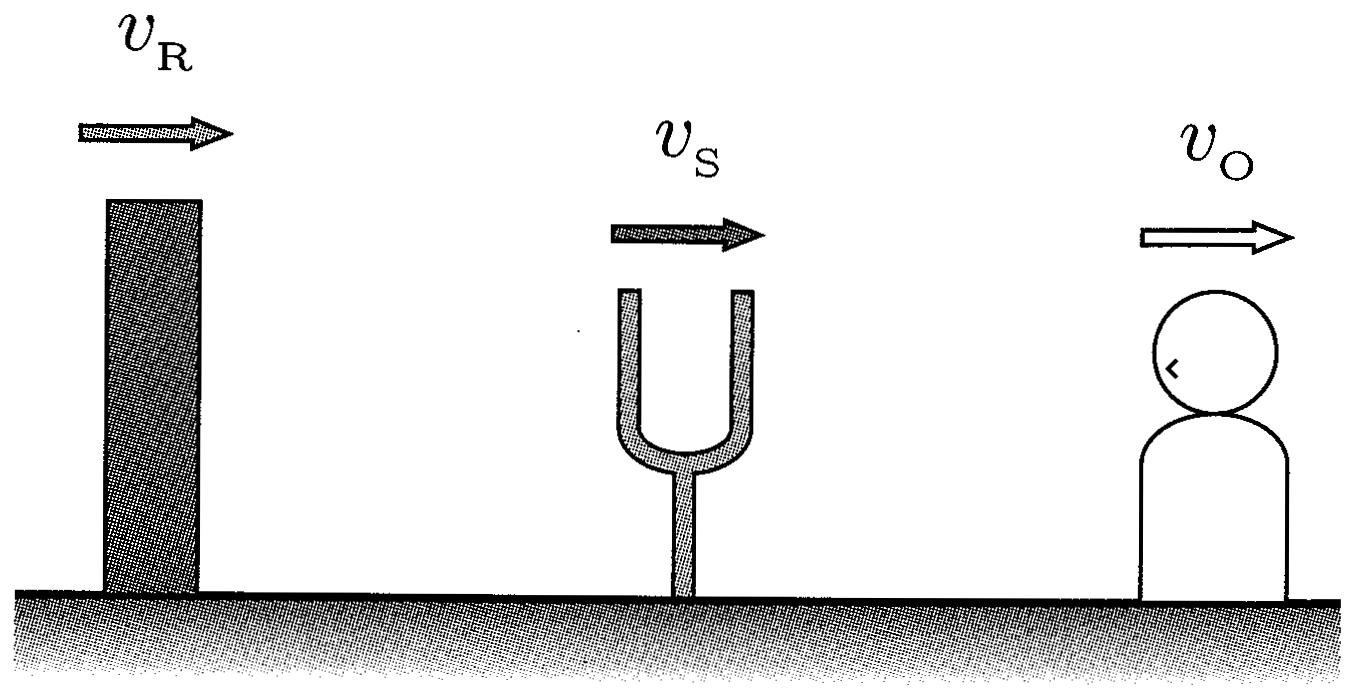
\includegraphics[keepaspectratio,width=68mm]{fig/n17_ex17_z.png}
\end{zuright}
\begin{komon}
\ko{1} 音源$\mathrm{S}$から観測者$\mathrm{O}$に直接やってくる音の振動数$f_1\U{Hz}$を求めよ．
\ko{2} 音源$\mathrm{S}$から反射壁$\mathrm{R}$で反射し，観測者$\mathrm{O}$に届く反射音の振動数$f_2\U{Hz}$を求めよ．
\end{komon}
\end{reidai}

\begin{sisinE}
\MARU{1}まず壁と共に運動する観測者を考え，この観測者が受け取る振動数$f^\prime\U{Hz}$を求める．
\MARU{2}壁を振動数$f^\prime\U{Hz}$を発しながら動く波源だと考えて，真の観測者が受け取る振動数$f^{\prime\prime}\U{Hz}$を求める．
\MARU{1}\MARU{2}の各段階でドップラー効果の関係式を用いて振動数を求めていけばよい．

{\gtfamily 直接音と反射音とでは音の進行方向が逆}であることに注意せよ．正の向きの取り方が段階ごとに変わる．
\end{sisinE}
\Key{壁による反射\quad $\Rightarrow$\quad \MARU{1}壁を観測者とみなす\quad \MARU{2}壁を波源とみなす，の2段階}

\begin{kaitou}
\begin{komon}
\ko{1} $\mathrm{S}$から$\mathrm{O}$へ向かう音は東向きに進むので，東向きを正とする．観測者$\mathrm{O}$の速度は$+v_\mathrm{O}$，波源$\mathrm{S}$の速度は$+v_\mathrm{S}$であるから，
       \Ana{f_1=\frac{c-v_\mathrm{O}}{c-v_\mathrm{S}}f_0\U{Hz}\Ans}
\ko{2} $\mathrm{S}$から$\mathrm{R}$へ向かう音は西向きに進むので，この段階では西向きを正とする．壁$\mathrm{R}$を観測者とみなすと，その速度は$-v_\mathrm{R}$，波源$\mathrm{S}$の速度は$-v_\mathrm{S}$であるから，壁が受け取る振動数$f^\prime\U{Hz}$は
       \Ana{f^\prime=\frac{c-(-v_\mathrm{R})}{c-(-v_\mathrm{S})}f_0=\frac{c+v_\mathrm{R}}{c+v_\mathrm{S}}f_0\U{Hz}}
       次に，壁$\mathrm{R}$を振動数$f^\prime\U{Hz}$の波源とみなす．反射音は東向きに進むので東向きを正とすると，波源（＝壁）の速度は$+v_\mathrm{R}$，観測者$\mathrm{O}$の速度は$+v_\mathrm{O}$であるから，
       \Ana{f_2=\frac{c-v_\mathrm{O}}{c-v_\mathrm{R}}f^\prime=\frac{(c-v_\mathrm{O})(c+v_\mathrm{R})}{(c-v_\mathrm{R})(c+v_\mathrm{S})}f_0\U{Hz}\Ans}
\end{komon}
\end{kaitou}
\begin{chuu}
壁が受け取った波の数と壁が送り出す波の数は等しい．だから壁は「振動数$f^\prime$の音源」として扱える．
壁が動いていても{\gtfamily 反射のときに振動数が変わるのではなく}，壁が受け取る段階と壁から出る段階の2回のドップラー効果が起きているのだと理解すること．
\end{chuu}
\end{reidaiunit}

\bsNeed{30mm}
\subsection{斜めドップラー効果}
\begin{wrapfigure}[9]{r}[5mm]{90mm}
  \centering
  \vspace{-5mm}
  
\includegraphics[keepaspectratio,width=90mm]
  {text_p113_fig1.png}
\end{wrapfigure}
ここまでは波源と観測者が，その2点を結ぶ直線方向のみに運動する場合を考えたが，それ以外の方向に波源・観測者が運動する場合は，波源と観測者の速度のうち，波の伝播方向の速度成分のみがドップラー効果に有効であることが知られている．

例えば，右図のように波源と観測者が運動する場合は，波の伝播方向の速度成分である$v\cos\theta\U{m/s}$および$u\cos\varphi\U{m/s}$がドップラー効果に有効な速度成分であるから，
\[f^\prime=\frac{c+u\cos\varphi}{c-v\cos\theta}f\U{Hz}\]
なる振動数の音が観測される．

% 加筆（2026-09-14 ユーザー指摘）：本文は「どちらも波の伝播方向の速度成分」としか書いて
%   いないが，原本の図（text_p113_fig1.png）では θ は「波源→観測者」の向きから，
%   φ は「観測者→波源」の向きから測っており，基準が180°違う。だから観測者側だけ符号が
%   ＋になる。素直に読むと (c−u cosφ)/(c−v cosθ) と書いてしまう（17.4 で
%   「(c−観測者の速度)/(c−波源の速度)」を習った直後なのでなおさら取り違える）。
\hspace{1zw}ここで，{\gtfamily 角を測る向きが波源側と観測者側で違う}ことに注意しなければならない．
右図をよく見ると，$\theta$は{\gtfamily 波源から観測者を見る向き}（＝波の伝播方向）から測っているのに対し，$\varphi$は{\gtfamily 観測者から波源を振り返る向き}（＝その逆向き）から測っている．
分母が$-$，分子が$+$と食い違って見えるのはこのためである．
実際，観測者がまっすぐ遠ざかる場合は$\varphi=180^\circ$で分子が$c-u$となって$f^\prime$は小さくなり，まっすぐ近づく場合は$\varphi=0^\circ$で分子が$c+u$となって$f^\prime$は大きくなる．これは 17.3 の結果と一致している．

% この注意は例題19の【注】にもあるが，公式の初出のここに無いと入試で取り違える
% （2026-09-05 追加）。
\hspace{1zw}ここで，{\gtfamily $\theta$は音を出した瞬間の波源の位置と観測点とを結ぶ方向から測る}ことに注意せよ（音が届いた瞬間の波源の位置ではない）．

\bsNeed{96mm}
%%%%%  例題18（17.7 の直後）＝ 原本【例題18】〈斜めドップラー効果〉（p113）  %%%%%%
\begin{reidaiunit}
\begin{reidai}{斜めドップラー効果}
\hspace{1zw}図に示すように，振動数$f\U{Hz}$の音源$\mathrm{S}$が，$\mathrm{O}$点を中心とする半径$R\U{m}$の円周上を一定の速さ$v\U{m/s}$で上から見て反時計まわりに運動している．この音源の音を，円周と同一平面上にあり，$\mathrm{O}$からの距離$l_1\U{m}$だけ離れた点$\mathrm{P_1}$で観測する．音速を$c\U{m/s}$，$v<c$，風はないものとする．

% 加筆（2026-09-14 ユーザー指摘）：原本は θ の定義を図だけに任せているが，直前の 17.7 で
%   別の意味の θ（速度と SP のなす角）を定義したばかりなので衝突する。問題文に
%   「∠SOP1 を θ とする」を補った（原本にない補筆。記号そのものは原本のまま θ）。
\hspace{1zw}このとき，点$\mathrm{P_1}$での観測音の振動数が最小になる音を出すときの音源の位置と，観測される振動数$f_{\min}\U{Hz}$を求めよ．ただし図のように，$\mathrm{OS}$と$\mathrm{OP_1}$のなす角を$\theta$とし，音源の位置は角$\theta$の余弦$\cos\theta$を与える式として示せ．
\begin{center}
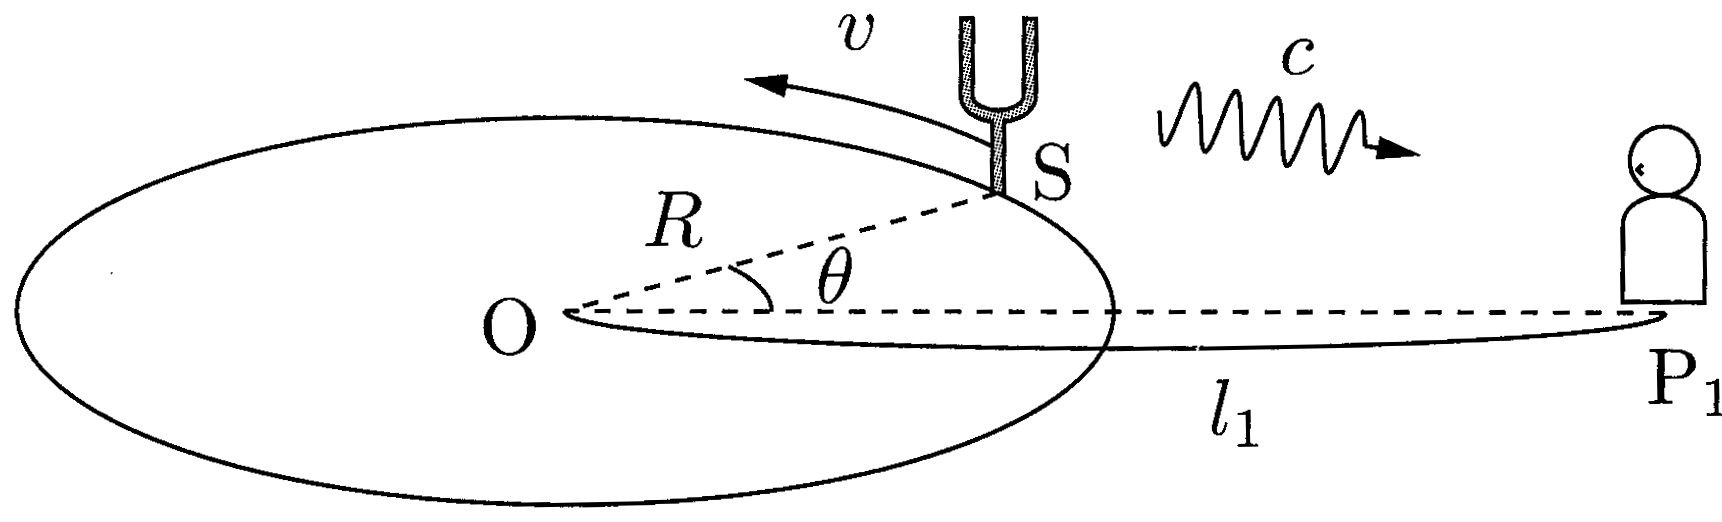
\includegraphics[keepaspectratio,width=105mm]{fig/n17_ex18_z.png}
\end{center}
\end{reidai}

\begin{sisinE}
まず{\gtfamily この問題の$\theta$は音源の「位置」を表す角}（円の中心$\mathrm{O}$から見た角$\angle\mathrm{SOP_1}$）であり，17.7 の斜めドップラー効果の式に現れる$\theta$（音源の速度と$\mathrm{SP_1}$のなす角）とは別物であることに注意する．

斜めドップラー効果では{\gtfamily 音の伝播方向（音源と観測者を結ぶ向き）の速度成分}だけが効く．
観測される振動数が最小になるのは，音源が$\mathrm{P_1}$から{\gtfamily 最も速く遠ざかる}ときである．

音源$\mathrm{S}$の速度は円の接線方向を向いているから，$\mathrm{SP_1}$方向の速度成分が最大の大きさで遠ざかる向きになるのは，{\gtfamily 速度ベクトルそのものが$\mathrm{P_1}$から遠ざかる向きに一直線に並ぶとき}，すなわち直線$\mathrm{SP_1}$が円に接するときである．
このとき遠ざかる速さはちょうど$v\U{m/s}$になる．
\end{sisinE}
\Key{斜めドップラー効果\quad $\Rightarrow$\quad 音の伝播方向の速度成分を取る}

\begin{kaitou}
\hspace{1zw}$\mathrm{S}$の速度は円の接線方向を向いており，その大きさは$v\U{m/s}$である．$\mathrm{SP_1}$方向の速度成分の大きさは$v$を超えないから，$\mathrm{P_1}$から遠ざかる速さが最大となるのは{\gtfamily 速度ベクトルが$\mathrm{P_1}$から遠ざかる向きの直線$\mathrm{SP_1}$上に乗るとき}，すなわち直線$\mathrm{SP_1}$が点$\mathrm{S}$で円に接するときである．

\hspace{1zw}このとき$\mathrm{OS}\perp\mathrm{SP_1}$であるから，直角三角形$\mathrm{OSP_1}$に着目して
\Ana{\cos\theta=\frac{R}{l_1}\Ans}
となる位置に音源があるときである（反時計まわりであるから，図の上側の接点）．
このとき音源は$\mathrm{P_1}$から速さ$v\U{m/s}$で遠ざかるので，
\Ana{f_{\min}=\frac{c}{c+v}f\U{Hz}\Ans}
\end{kaitou}
\begin{chuu}
同様に，観測される振動数が最大になるのは下側の接点（$\cos\theta=\dfrac{R}{l_1}$かつ$\mathrm{P_1}$に近づく向き）を音源が通過するときで，そのときの振動数は$\dfrac{c}{c-v}f\U{Hz}$である．
一方，音源が$\mathrm{OP_1}$の延長線上（$\theta=0^\circ$, $180^\circ$）にあるときは速度が$\mathrm{SP_1}$と垂直になるので，そのとき出された音はドップラー効果を受けず$f\U{Hz}$のまま観測される．
\end{chuu}
\end{reidaiunit}

\bsNeed{46mm}
\subsection{斜めドップラー効果の式の導出問題}

斜めドップラー効果の式を導くには，微小時間の間に波源が出す波を観測者が受け取る時間間隔を考えることにより算出するという方法がある．

\bsNeed{100mm}
%%%%%  例題19（17.8 の直後）＝ 原本【例題19】〈斜めドップラー効果の導出〉（p114）  %%%%%%
\begin{reidaiunit}
\begin{reidai}{斜めドップラー効果の導出}
\begin{zuright}{50mm}
\hspace{1zw}一定の速さ$v\U{m/s}$で直線上を運動している振動数$f\U{Hz}$の音源が，点$\mathrm{O}$を通過する瞬間から微小時間$\Delta t\U{s}$の間に発する音について考える．$\mathrm{O}$から見て音源の運動方向と角$\theta$，距離$r\U{m}$だけ離れた図の$\mathrm{P}$点でこの音を聞く．音速を$c\U{m/s}$（ただし$v<c$），また音源が微小時間$\Delta t\U{s}$の間に動く距離$v\cdot\Delta t\U{m}$は$r$に比べて十分小さいとして以下の問に答えよ．
\zusep
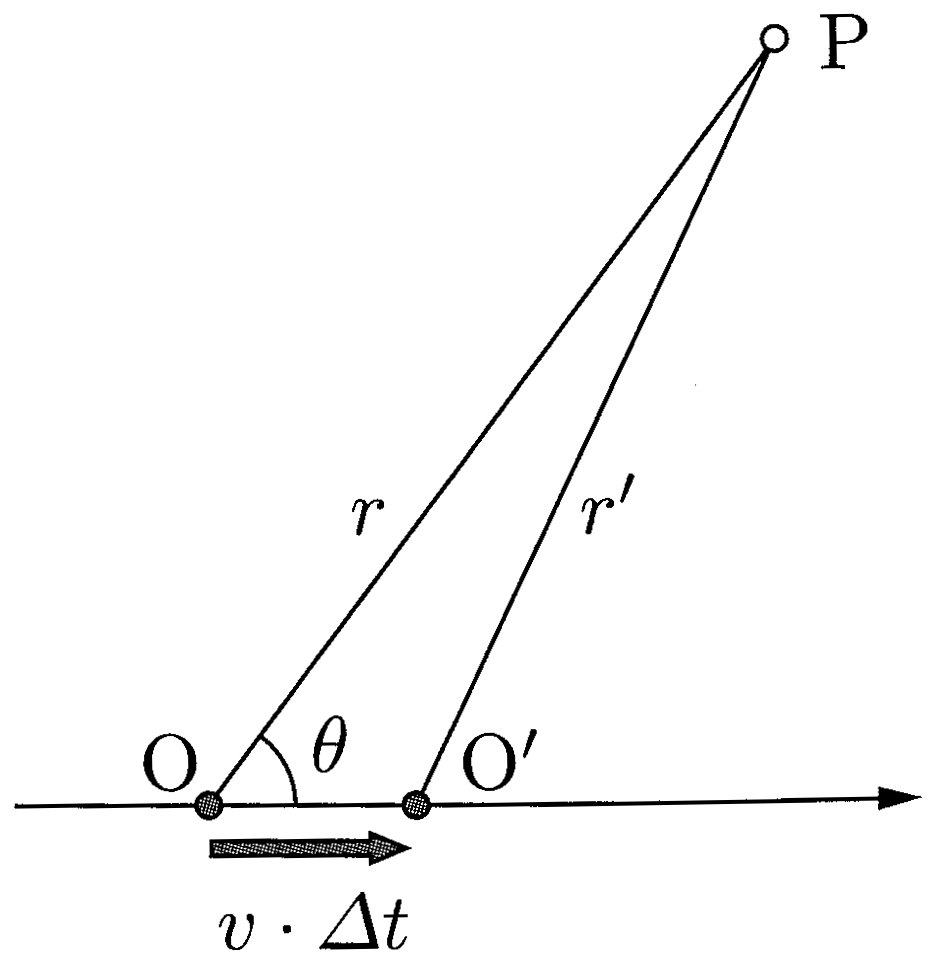
\includegraphics[keepaspectratio,width=50mm]{fig/n17_ex19_z.png}
\end{zuright}
\begin{komon}
\ko{1} 音源が，点$\mathrm{O}$を通過してから$\Delta t\U{s}$後にいる位置を$\mathrm{O}^\prime$とする．このとき，$\mathrm{O}^\prime\mathrm{P}$間の距離$r^\prime\U{m}$は近似的に$r-v\Delta t\cos\theta\U{m}$で与えられることを示せ．
\ko{2} 音源が点$\mathrm{O}$を通過する時刻を$t=0\U{s}$とするとき，$\mathrm{O}$点から来る音が$\mathrm{P}$点に達する時刻$t_1\U{s}$および$\mathrm{O}^\prime$点から来る音が$\mathrm{P}$点に達する時刻$t_2\U{s}$を求めよ．
\ko{3} 微小時間$\Delta t\U{s}$の間に音源が出す音波の山の数はいくつか．
\ko{4} $\mathrm{O}$点から発せられた音が点$\mathrm{P}$で観測されるときの振動数$f^\prime\U{Hz}$を$f,c,v,\theta$を用いて表せ．
\end{komon}
\end{reidai}

\begin{sisinE}
音波が伝わるのに要する時間，図の各点に達する時刻をきちんと分けて扱うこと．

$\Delta t\U{s}$の間に出た$f\Delta t$個の波は，$\mathrm{P}$点では$t_1$から$t_2$までの間に受け取られる．
{\gtfamily 観測される振動数は「受け取る波の数」÷「受け取るのに要した時間」}であるから，$f^\prime=\dfrac{f\Delta t}{t_2-t_1}$である．
\end{sisinE}
\Key{$f^\prime=\dfrac{\text{微小時間に出た波の数}}{\text{それを受け取るのに要する時間}}$}

\begin{kaitou}
\begin{komon}
\ko{1} 三角形$\mathrm{OO^\prime P}$に余弦定理を用いると，
       \[{r^\prime}^2=r^2+(v\Delta t)^2-2r\cdot v\Delta t\cos\theta\]
       $v\Delta t$は$r$に比べて十分小さいので$(v\Delta t)^2$の項を無視すると，
       \[{r^\prime}^2=r^2\left(1-\frac{2v\Delta t\cos\theta}{r}\right)\]
       $|x|\ll1$のとき$\sqrt{1+x}\fallingdotseq1+\dfrac{x}{2}$であるから，
       \Ana{r^\prime\fallingdotseq r\left(1-\frac{v\Delta t\cos\theta}{r}\right)=r-v\Delta t\cos\theta\U{m}}
\ko{2} $\mathrm{O}$点から出た音は$t=0$に発せられて距離$r$を進むから，
       \Ana{t_1=\frac{r}{c}\U{s}\Ans}
       $\mathrm{O}^\prime$点から出た音は$t=\Delta t$に発せられて距離$r^\prime$を進むから，
       \Ana{t_2=\Delta t+\frac{r^\prime}{c}=\Delta t+\frac{r-v\Delta t\cos\theta}{c}\U{s}\Ans}
\ko{3} 振動数$f\U{Hz}$の音源が$\Delta t\U{s}$の間に出す波の数であるから，
       \Ana{f\Delta t\ \text{個}\Ans}
\ko{4} $\mathrm{P}$点の観測者は，時刻$t_1$から$t_2$までの間に$f\Delta t$個の波を受け取る．
       \[t_2-t_1=\Delta t+\frac{r-v\Delta t\cos\theta}{c}-\frac{r}{c}=\frac{c-v\cos\theta}{c}\Delta t\]
       であるから，
       \Ana{f^\prime=\frac{f\Delta t}{t_2-t_1}=\frac{c}{c-v\cos\theta}f\U{Hz}\Ans}
\end{komon}
\end{kaitou}
\begin{chuu}
観測者も動く場合は，観測者が波を受け取る側でさらに$\mathrm{P}$点が移動するので，同じ議論を繰り返して
$f^\prime=\dfrac{c+u\cos\varphi}{c-v\cos\theta}f\U{Hz}$が得られる．
$\theta$は{\gtfamily 音を出した瞬間}の位置と観測点を結ぶ方向から測ることに注意せよ（音が届いた瞬間の位置ではない）．
\end{chuu}
\end{reidaiunit}

\bsNeed{100mm}
\subsection{衝撃波}
\begin{wrapfigure}[19]{r}[5mm]{65mm}
  \centering
  \vspace{-5mm}
  
\includegraphics[keepaspectratio,width=65mm]
  {text_p115_fig1.png}
\end{wrapfigure}
今まで考えてきたドップラー効果はいずれも波源の速さが波の速さを超えない場合であった．
もし波源の速さが波の速さを超えるようになると，波源の前方へ進む波の波長はドップラー効果の式から計算すると負になってしまう．
これは，$v>c$ではもはや{\gtfamily 波源が自分の出した波よりも先へ進んでしまい，前方に一定波長の波列ができるという今までの考え方が使えなくなった}ことを意味している．実際に波面を作図して確かめてみよう．

音源$\mathrm{S}$の速さが$v\U{m/s}$，音速が$c\U{m/s}$とし，$v>c$の条件が満たされている場合について考えると，図$\fbox{1}$の$\mathrm{P_1}$を通過したときに出た音波は$\mathrm{P_1}$を中心として同心円状に広がる．
やがて$\mathrm{P_2}$に音源は達するが，このときの$\mathrm{P_1}$を通過したときに出された音波の波面は図$\fbox{2}$のようになっている．
$\mathrm{P_2}$を通過するときに出す音波は通過したときから$\mathrm{P_2}$を中心として同心円状に広がっていく．
これを繰り返していくと，各$\mathrm{P_1}$，$\mathrm{P_2}$，$\mathrm{P_3}$などから出た音波は図のような円錐形の波面を作ることになる．
% 加筆（2026-09-14 ユーザー指摘）：「図のような円錐形の波面を作る」「図より sinθ=c/v」と
%   図に任せきりで，なぜ円錐面が波面になるのか・なぜ ct が対辺なのかが読み取れなかった。
%   第14回 14.7 のホイヘンスの原理（包絡面）と結びつける。
この円錐面は，各点から出た球面波のすべてに共通に接する面であり，第14回 14.7 で述べたホイヘンスの原理の{\gtfamily 包絡面}にほかならない．
波面上には各時刻に出された球面波が重なり合うため，非常に大きな振幅を持つ波面となる．
このような波を{\gtfamily 衝撃波}という．

$\mathrm{P_1}$を通過してから時間$t\U{s}$だけ経過したときを考えると，$\mathrm{P_1}$から出た音波は半径$c\cdot t\U{m}$の球面に広がっており，一方で音源は$v\cdot t\U{m}$だけ進んで現在の位置にいる．
波面はこの球面に接しているので，接点と$\mathrm{P_1}$を結ぶ半径$c\cdot t\U{m}$は{\gtfamily 波面（円錐の母線）に垂直}である．
したがって斜辺$v\cdot t\U{m}$，$\theta$に対する対辺$c\cdot t\U{m}$の直角三角形ができ，衝撃波の半頂角を$\theta$として
\[\sin\theta=\frac{c\cdot t}{v\cdot t}=\frac{c}{v}\]
という関係が満たされる．
衝撃波においては，波源の進行方向の波源より前方には波は伝わっていかず，波源の後方へ進む波については通常のドップラー効果が観測される．

\begin{matome}{衝撃波}
\hspace{3mm} 波源の速さが波の速さを超えると，波源の進行方向の波源より前方には波は伝わっていかない．\\
\hspace{3mm} 波源から出る波の波面は波源を頂点とする円錐形をなし，その半頂角$\theta$は$\sin\theta=\dfrac{c}{v}$を満たす．
\end{matome}


\newpage

% 練習番号：第16回で［21］〜［28］を使ったのでこの回は［29］から
\setcounter{qno}{28}

\filbreak
\Rank{A問題}

\Mon{基本事項の確認}

\hspace{1zw}音速を$340\U{m/s}$として，以下の設問に答えよ．特に指示がない限り，答えはすべて小数第1位まで求めよ．
\begin{komon}
\ko{1} 振動数$400\U{Hz}$の音を出しながら速さ$20\U{m/s}$で進んでいる音源がある．音源の進行方向の前方へ進んだ音の波長は何$\U{m}$か．また音源の進行方向の後方へ出た音の波長は何$\U{m}$か．
\ko{2} 振動数$440\U{Hz}$の音を出して静止している音源がある．この音源から速さ$10\U{m/s}$で遠ざかる観測者の聞く音の振動数は何$\U{Hz}$か．またこの音源に向かって速さ$10\U{m/s}$で近づいている観測者の聞く音の振動数は何$\U{Hz}$か．
\ko{3} 振動数$400\U{Hz}$の音を出して速さ$20\U{m/s}$で進んでいる音源がある．この音源の進む前方から速さ$10\U{m/s}$で近づいている観測者の聞く音の振動数は何$\U{Hz}$か．
\ko{4} 振動数$440\U{Hz}$の音源を，壁に向かって速さ$10\U{m/s}$で近づけるとき，音源の後方に静止している観測者に直接やってくる音の振動数は何$\U{Hz}$か．また壁で反射して観測者に届く音の振動数は何$\U{Hz}$か．
\ko{5} 振動数$400\U{Hz}$の音を出しながら速さ$20\U{m/s}$で進んでいる音源がある．音源の動く向きと同じ向きに風速$5\U{m/s}$の風が吹いているとき，音源の進む前方での音の波長は何$\U{m}$か．また音源の進む後方での音の波長は何$\U{m}$か．答えはすべて小数第2位まで求めよ．
\end{komon}
% 統合（2026-09-05）：原本 第23回のA問題［30］（1)(2)(3)と［31］(1)(2)を1題にまとめた．
%   設問は1つも落としていない（［30］(1)(2)(3)＝(1)(2)(3)，［31］(1)(2)＝(4)(5)）．
% 誤植訂正：原本［31］(2)は「風速 5[m] の風」．[m] は [m/s] の誤り．

\filbreak
\Rank{B問題}

\Mon{音源が媒質に対して動く場合のドップラー効果}

\begin{zuright}{58mm}
\hspace{1zw}$\mathrm{A}$の地点にマイクを取り付け，$\mathrm{A}$で受け取った音を$\mathrm{B}$地点へ電送するような装置を用意する．今，$\mathrm{A}$から$\mathrm{B}$に向けて進む音源が$128\U{Hz}$の音を出したとき，$\mathrm{B}$にいる人が毎秒2回のうなりを聞いた．音の伝わる速さが$340\U{m/s}$であるとして，音源の移動する速さを有効数字3桁で求めよ．必要ならば，$|x|\ll1$について成り立つ近似式$\dfrac{1}{1\pm x}\fallingdotseq1\mp x$（複号同順）を用いてよい．
\zusep
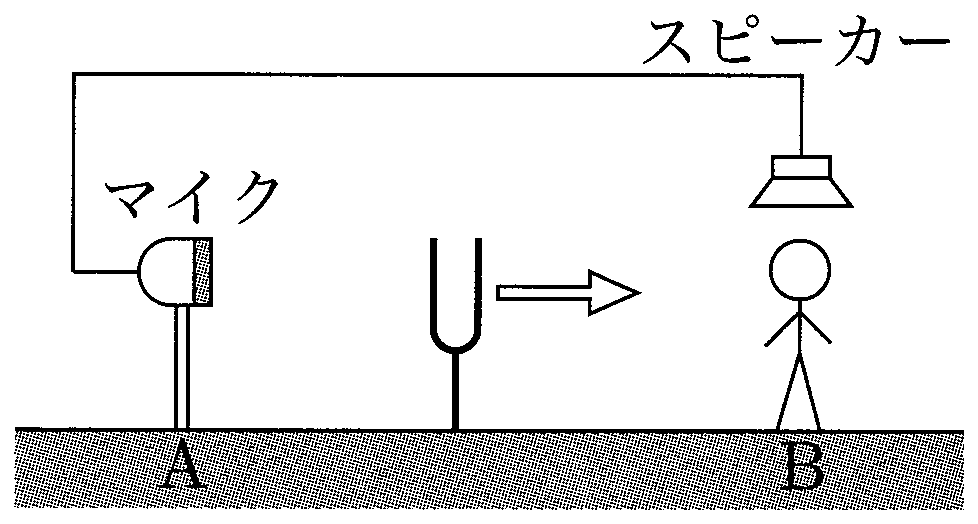
\includegraphics[keepaspectratio,width=58mm]{fig/n17_p30_mic.png}
\end{zuright}

\Mon{列車のドップラー効果}

\begin{zuright}{52mm}
\hspace{1zw}直線状の線路を一定の振動数の警笛を鳴らしながら列車が等速度で進行している．線路の近くで同じ側の2点にマイクロホン$\mathrm{A}$, $\mathrm{B}$を置き，受けた音の振動数を測定した．図には観測された振動数が時刻に対してどのような変化をしたのかを$\mathrm{A}$, $\mathrm{B}$それぞれについて示してある．警笛の振動数を$200\U{Hz}$，音速を$340\U{m/s}$，図の$t_\mathrm{B}-t_\mathrm{A}=8\U{s}$，またマイクロホン$\mathrm{A}$, $\mathrm{B}$間の距離は$40\U{m}$である．以下の設問に答えよ．
\begin{komon}
\ko{1} 列車の速さを求めよ．
\ko{2} 図中の振動数$f_1$, $f_2$を求めよ．
\end{komon}
\zusep
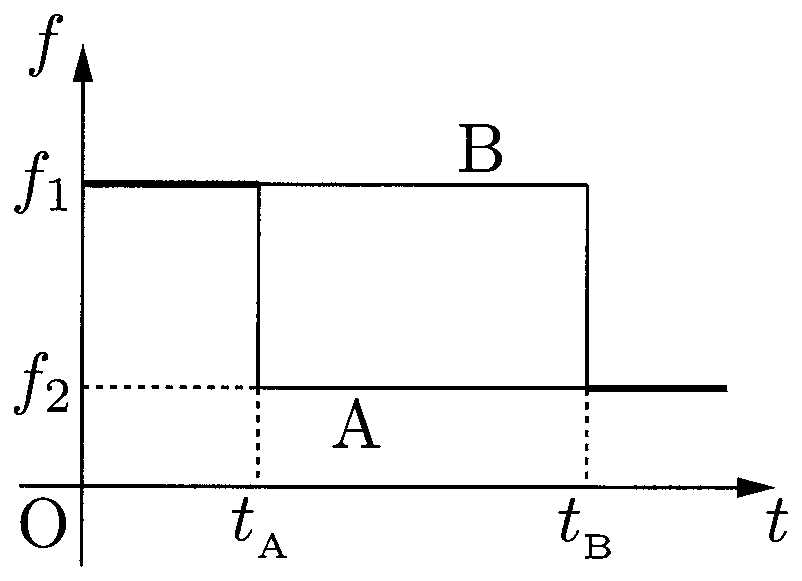
\includegraphics[keepaspectratio,width=52mm]{fig/n17_p31_graph.png}
\end{zuright}
% 誤植訂正（2026-09-05）：原本は「マイクロホン A, B 間の距離は 40[cm]」だが，
%   解答は「距離 40[m] だけ離れたマイク A, B」として $v=40/8=5$[m/s] を出している．[m] が正しい．

\Mon[\Sitei]{空間中に広がるドップラー効果}

\begin{zuright}{50mm}
\hspace{1zw}平面上で音源$\mathrm{A}$から振動数$f\U{Hz}$の音波が放射されている．$\mathrm{A}$から見て東の方向に振動数を測定する装置$\mathrm{B}$を置いた．媒質を伝わる音の速さを$V\U{m/s}$，風はないものとして，以下の空欄\framebox[3zw]{\rule{0pt}{1.1zw}}の中に当てはまる適当な式を求めよ．
\zusep
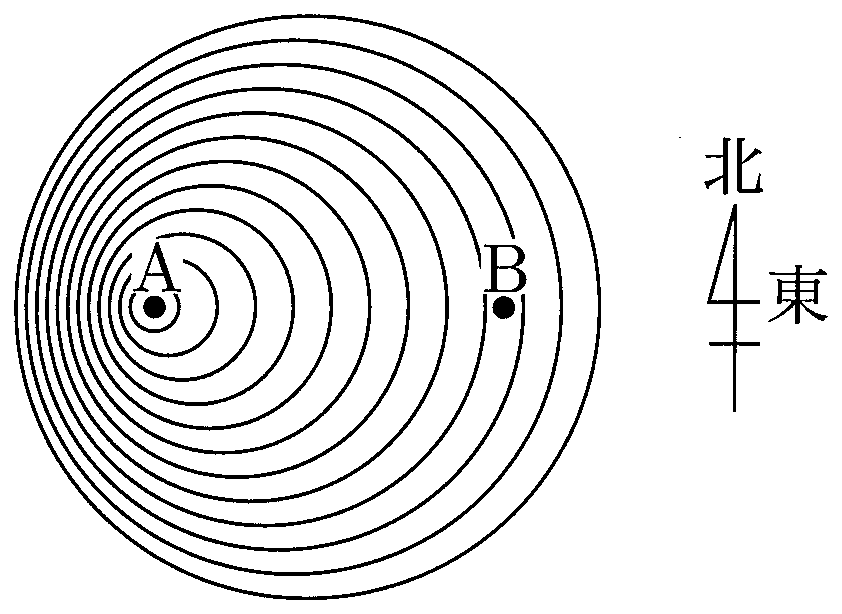
\includegraphics[keepaspectratio,width=50mm]{fig/n17_p32_hamen.png}
\end{zuright}
\hspace{1zw}ある瞬間に図のような波面が見られた．この波面の形から波源$\mathrm{A}$は，\fbox{1}向きに進んでいることがわかる．波源$\mathrm{A}$の速さを$v\U{m/s}$とすれば，$\mathrm{A}$から東に向かう波の波長は\fbox{2}であるから，装置$\mathrm{B}$が静止している場合には，測定される振動数は\fbox{3}となる．また，$\mathrm{A}$の速度はそのままで，$\mathrm{B}$が速さ$u\U{m/s}$で西向きに移動している場合には，$\mathrm{B}$で測定される振動数は\fbox{4}となる．

\Mon{一直線上のドップラー効果}

\hspace{1zw}直線状道路で車を$80\U{km/h}$で走らせていたところ，道路の横に平行している線路の前方から超特急がやってきて，後方へと走り去って行った．このとき，超特急が発していた警笛の最初の音の振動数は，走り去った後の音の振動数の$\dfrac{8}{5}$倍であったという．音速を$1200\U{km/h}$として以下の設問に答えよ．
\begin{komon}
\ko{1} この超特急の速さを求めよ．
\ko{2} このとき，道路にたたずんでいる人がこの警笛を聞いた．超特急が通過した前後の音の振動数の比を求めよ．
\end{komon}

\Mon{ドップラー効果とうなり}

\begin{zuright}{58mm}
\hspace{1zw}二つのスピーカー$\mathrm{A}$, $\mathrm{B}$を向かい合わせに置き，その間に観測者$\mathrm{O}$が静止している．$\mathrm{A}$, $\mathrm{B}$から音を出すと，1秒間あたりに$N$回のうなりが観測されたが，$\mathrm{B}$をある一定の速さで遠ざけたところ，うなりが観測されなくなった．以下の設問に答えよ．ただしこの温度における音速を$c\U{m/s}$とし，$\mathrm{A}$から出る音の振動数を$f\U{Hz}$とする．
\zusep
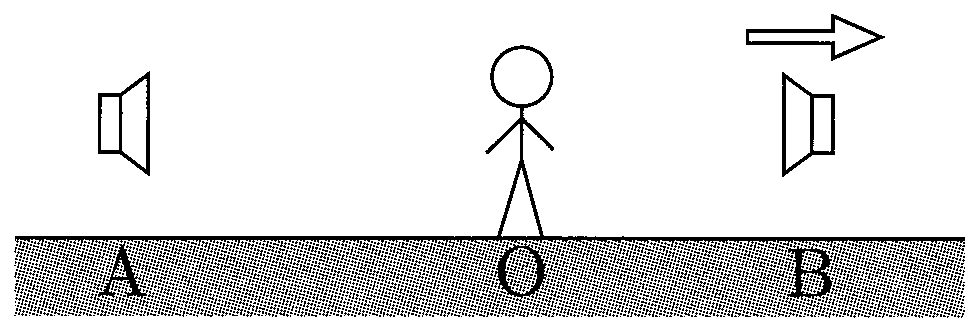
\includegraphics[keepaspectratio,width=58mm]{fig/n17_p34_speaker.png}
\end{zuright}
\begin{komon}
\ko{1} $\mathrm{B}$から出ている音の振動数$f^\prime\U{Hz}$を求めよ．
\ko{2} うなりが観測されなくなったときの$\mathrm{B}$の速さ$v\U{m/s}$を求めよ．
\ko{3} $\mathrm{A}$, $\mathrm{B}$が静止しているとき，$\mathrm{O}$が運動してうなりが観測されなくなるための$\mathrm{O}$の速度を求めよ．
\end{komon}

\Mon[\Sitei]{反射波によるドップラー効果および風の効果}

\begin{zuright}{58mm}
\hspace{1zw}一直線上に，図のように観測者$\mathrm{O}$，振動数$f\U{Hz}$の音源$\mathrm{S}$，壁$\mathrm{R}$が並んでいる．観測者$\mathrm{O}$は右向きに速さ$u\U{m/s}$で，壁$\mathrm{R}$は左向きに速さ$V\U{m/s}$で運動しており，図の左から右へ向かって風速$w\U{m/s}$の風が吹いている．この温度における音速を$c\U{m/s}$とし，$u,V<c$であるとして以下の設問に答えよ．
\begin{komon}
\ko{1} 音源$\mathrm{S}$から観測者$\mathrm{O}$に直接やってくる音の振動数$f_1\U{Hz}$を求めよ．
\ko{2} 音源$\mathrm{S}$から壁$\mathrm{R}$で反射し，観測者$\mathrm{O}$に届く反射音の振動数$f_2\U{Hz}$を求めよ．
\end{komon}
\zusep
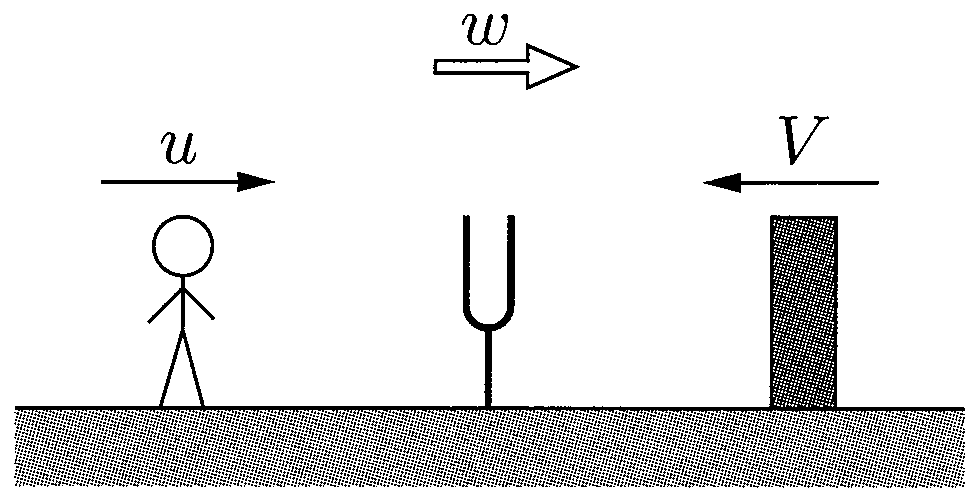
\includegraphics[keepaspectratio,width=58mm]{fig/n17_p35_wind.png}
\end{zuright}
% 誤植訂正（2026-09-05）：原本の本文は「$u, v<c$である」だが，図でも解答でも壁の速さは $V$．
%   小文字の $v$ はこの問題には登場しないので $V$ に直した．

\Mon{直接音と反射音によるうなり}

\begin{zuright}{54mm}
\hspace{1zw}図のようにスピーカー$\mathrm{S}$，マイクロホン$\mathrm{M}$，反射壁$\mathrm{R}$を一直線上に配置する．スピーカーは常に一定の振動数$f_0\U{Hz}$の音波を出し続けている．マイクロホンは音の強弱の変化を敏感に捉えることができ，反射壁は音をよく反射する．また，風は吹いていない．この状態において，以下の二つの実験を行った．
\zusep
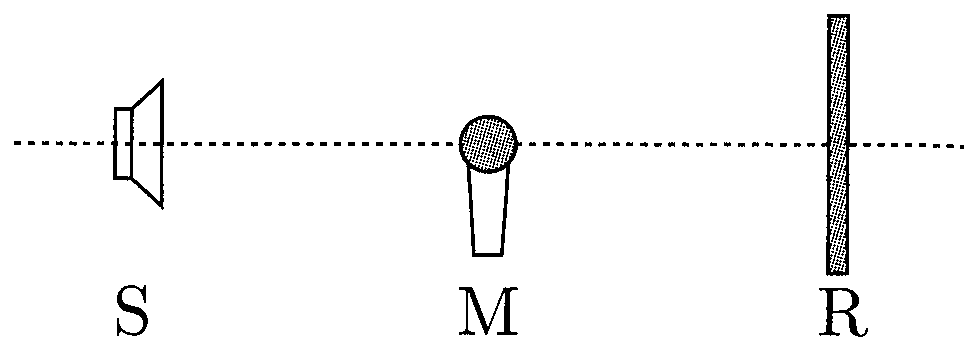
\includegraphics[keepaspectratio,width=54mm]{fig/n17_p36_smr.png}
\end{zuright}
\begin{description}
\item[実験\MARU{1}：] $\mathrm{S}$と$\mathrm{R}$を固定し，$\mathrm{M}$を一定の速さ$v\U{m/s}$で$\mathrm{R}$に近づける．
\item[実験\MARU{2}：] $\mathrm{R}$を固定し，$\mathrm{M}$と$\mathrm{S}$を一定の速さ$u\U{m/s}$で$\mathrm{R}$に近づける．
\end{description}
\hspace{1zw}いずれの場合も，$\mathrm{S}$, $\mathrm{R}$, $\mathrm{M}$の移動する速さは音速に比べて小さい．これらの実験に関して，以下の設問に答えよ．
\begin{komon}
\ko{1} 実験\MARU{1}で，マイクロホンのキャッチした音は，時間$t_1\U{s}$ごとに強から弱を経て強となる変化を繰り返した．このことを元に，このときの音速$c\U{m/s}$を求めよ．
\ko{2} 実験\MARU{2}で，マイクロホンのキャッチした音は，時間$t_2\U{s}$ごとに強から弱を経て強となる変化を繰り返した．$t_2\U{s}$を求めよ．
\end{komon}

\Mon[\Sitei]{斜めドップラー効果}

\begin{zuright}{58mm}
\hspace{1zw}直線$\mathrm{XY}$上を，振動数$f_0\U{Hz}$の音源$\mathrm{S}$が速さ$v\U{m/s}$で$\mathrm{X}$から$\mathrm{Y}$へ向かう向きに進んでいる．これを，図の$\mathrm{A}$点において観測する場合について以下の設問に答えよ．ただし音速を$c\U{m/s}$とし，$v\ll c$であるとする．
\zusep
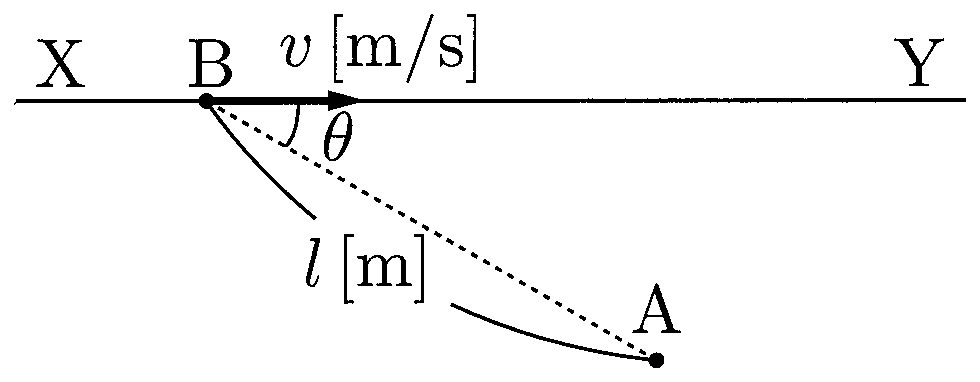
\includegraphics[keepaspectratio,width=58mm]{fig/n17_p37_xy.png}
\end{zuright}
\begin{komon}
\ko{1} $\mathrm{A}$点から距離$l\U{m}$，角度$\theta$の位置にある$\mathrm{B}$点において$\mathrm{S}$の出した音波が$\mathrm{A}$点に届いたとき，観測者が観測する音の振動数を$f_0,c,v,\theta$を用いて表せ．
\ko{2} 音源$\mathrm{S}$が$\mathrm{X}$の無限遠方から$\mathrm{Y}$の無限遠方に去っていくとき，$\mathrm{A}$点において観測される振動数は最初に聞こえ始めた振動数の$\dfrac{1}{3}$に減少した．このことを元に，音源の速さ$v$を求めよ．
\end{komon}

\Mon{斜めドップラー効果と音の伝わる速さ}

\begin{zuright}{50mm}
\hspace{1zw}右図のように，無風な平面上で，半径$500\U{m}$の水平面内の円軌道を，振動数$400\U{Hz}$の爆音を出しながら速さ$50\U{m/s}$で等速円運動している車がある．今，円軌道の中心$\mathrm{O}$から距離$1000\U{m}$だけ離れた$\mathrm{P}$点にいる観測者がこの爆音を聞くときについて，以下の設問に答えよ．ただし，音速を$350\U{m/s}$とする．
\zusep
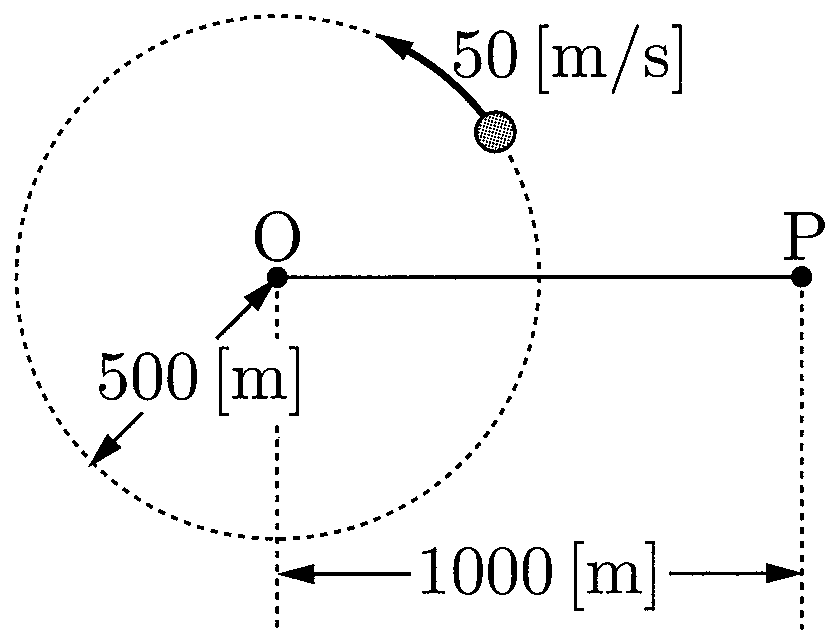
\includegraphics[keepaspectratio,width=50mm]{fig/n17_p38_circle.png}
\end{zuright}
\begin{komon}
\ko{1} この観測者の聞く音の振動数の最大値および最小値をそれぞれ求めよ．
\ko{2} この観測者がある瞬間に$400\U{Hz}$の爆音を聞き，その後，観測する振動数が単調に減少して(1)で求めた最小値になったという．$400\U{Hz}$の爆音を聞いてから最小の振動数の音を聞くまでに要した時間を求めよ．
\end{komon}

\filbreak
\Rank{C問題}

\Mon{ドップラー効果}

\hspace{1zw}直線道路を走る自動車に乗った観測者が救急車のサイレン音を聞いたため，車を止めて救急車が追い越していくのを待った．このとき，救急車のサイレン音は$1260\U{Hz}$から$1092\U{Hz}$へと変化した．救急車の速さおよび救急車から発せられるサイレン音の振動数は一定であり，音速は$336\U{m/s}$であるとする．以下の設問に答えよ．
\begin{komon}
\ko{1} 救急車の速さおよびサイレン音の振動数を求めよ．
\ko{2} 救急車から自動車にやってくるサイレン音の波長は，追い越す前および後でそれぞれどれだけか．
\ko{3} 救急車が通りすぎたので，観測者は救急車と同じ速さで救急車を追いかけた．このとき観測者が聞くサイレン音の振動数はいくらか．
\ko{4} (3)のとき，救急車が途中で止まったため，観測者の車は救急車を追い越した．救急車が止まった後のサイレン音の波長は，追い越し前と追い越し後とでそれぞれいくらか．ただし，観測者の車の速さは一定である．
\ko{5} (4)の後，救急車が動き出したため，観測者が聞くサイレン音の振動数が$1040\U{Hz}$になった．救急車はどちら向きにどれだけの速さで走り出したか．
\end{komon}

\Mon{ドップラー効果と気柱振動}

\begin{zuright}{50mm}
\hspace{1zw}長さ$l\U{m}$の閉管の軸上の開端の側で，周波数$f\U{Hz}$の音波を出す音源$\mathrm{S}$を動かす場合について考える．空気中の音速を$v\U{m/s}$として，以下の各設問に答えよ．
\zusep
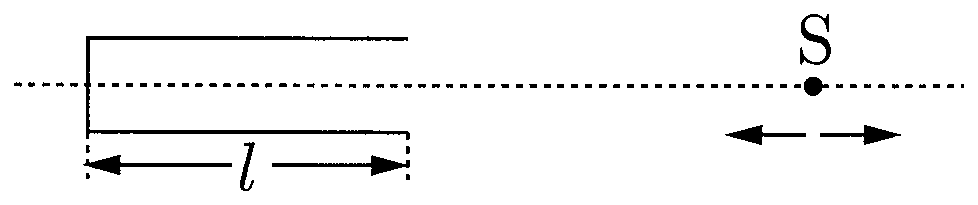
\includegraphics[keepaspectratio,width=50mm]{fig/n17_p40_tube.png}
\end{zuright}
\begin{komon}
\ko{1} $\mathrm{S}$を管の開端から遠ざけるとき，その速さを$0\U{m/s}$から次第に増していくと，速さ$u_1\U{m/s}$のとき，はじめて管内の気柱と共鳴し，これは$2m-1$倍振動であった．この条件から，$l,v,u_1,f,m$の間に成り立つ等式を示せ．
\ko{2} 今度は逆に$\mathrm{S}$を近づけるとき，速さを$0\U{m/s}$から次第に増していくと，速さ$u_2\U{m/s}$のとき，はじめて気柱の振動と共鳴した．(1)で用いた$m$と$l,v,u_2,f$の間に成立する等式を示せ．
\ko{3} $v=336\U{m/s}$, $f=3230\U{Hz}$, $u_1=25\U{m/s}$, $u_2=13\U{m/s}$のとき，$m$および気柱の長さ$l\U{m}$を求めよ．
\end{komon}

\Mon{斜めドップラー効果と音の伝わる速さ}

\begin{zuright}{56mm}
\hspace{1zw}飛行機が，観測者の真上を通る直線コースを一定の速さで水平飛行している．右のグラフは，飛行機が観測者の真上を通過した時刻を$0\U{s}$として，観測される飛行機音の振動数の時刻に対する変化を測定し，グラフ化したものである．風はなく，音速は$340\U{m/s}$であった．このグラフを読み取って，以下の設問に答えよ．
\zusep
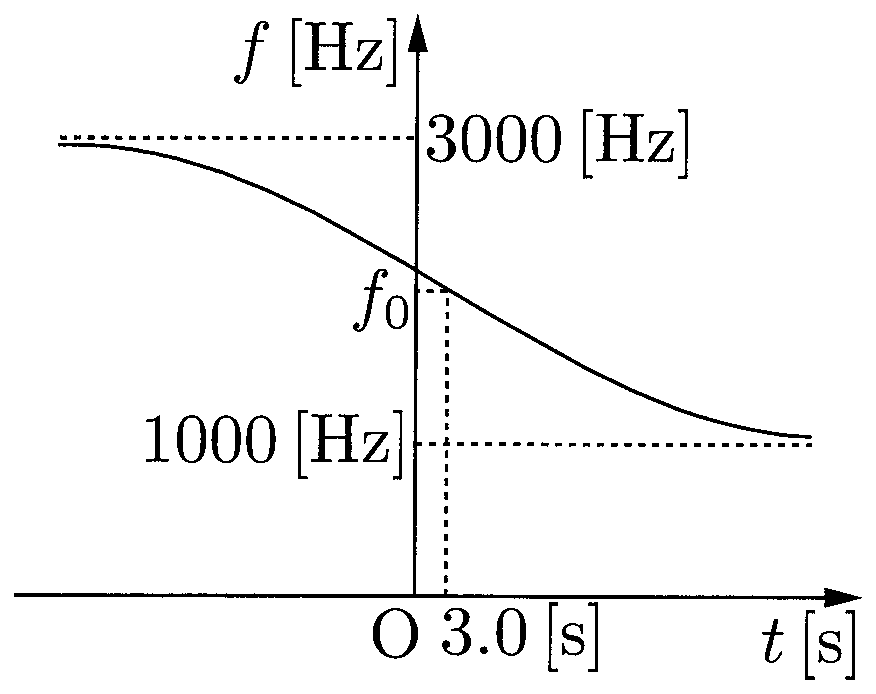
\includegraphics[keepaspectratio,width=56mm]{fig/n17_p41_graph.png}
\end{zuright}
\begin{komon}
\ko{1} 飛行機の真の振動数$f_0\U{Hz}$および飛行機の飛行する速さ$v\U{m/s}$を求めよ．
\ko{2} この観測者が時刻$3.0\U{s}$に飛行機の真の振動数$f_0\U{Hz}$を観測した．飛行機の高度を求めよ．
\ko{3} 時刻$0\U{s}$において観測者が聞いた音の振動数はいくらか．
\end{komon}

\Mon{衝撃波}

\hspace{1zw}音源が移動する場合の音波に関する以下の文章について，空欄を適当な文字，不等号などで埋めよ．

\hspace{1zw}音源$\mathrm{A}$が無風の空気中を等速直線運動している．$\mathrm{A}$が発する音波（振動数$f\U{Hz}$）は速さ$c\U{m/s}$で伝わり，$\mathrm{A}$自身は速さ$v\U{m/s}$で進んでいる．図(a), (b), (c)は$\mathrm{A}$の発する音波が伝わる様子を模式的に示している．$\mathrm{A}$は$1\U{s}$前に各図の$\mathrm{P}$の位置にあり，現在$\mathrm{Q}$の位置にある．いずれの図においても大きい円は$\mathrm{P}$で出た球面波を示し，小さい円は$0.5\U{s}$前に出た球面波を示している．
\begin{center}
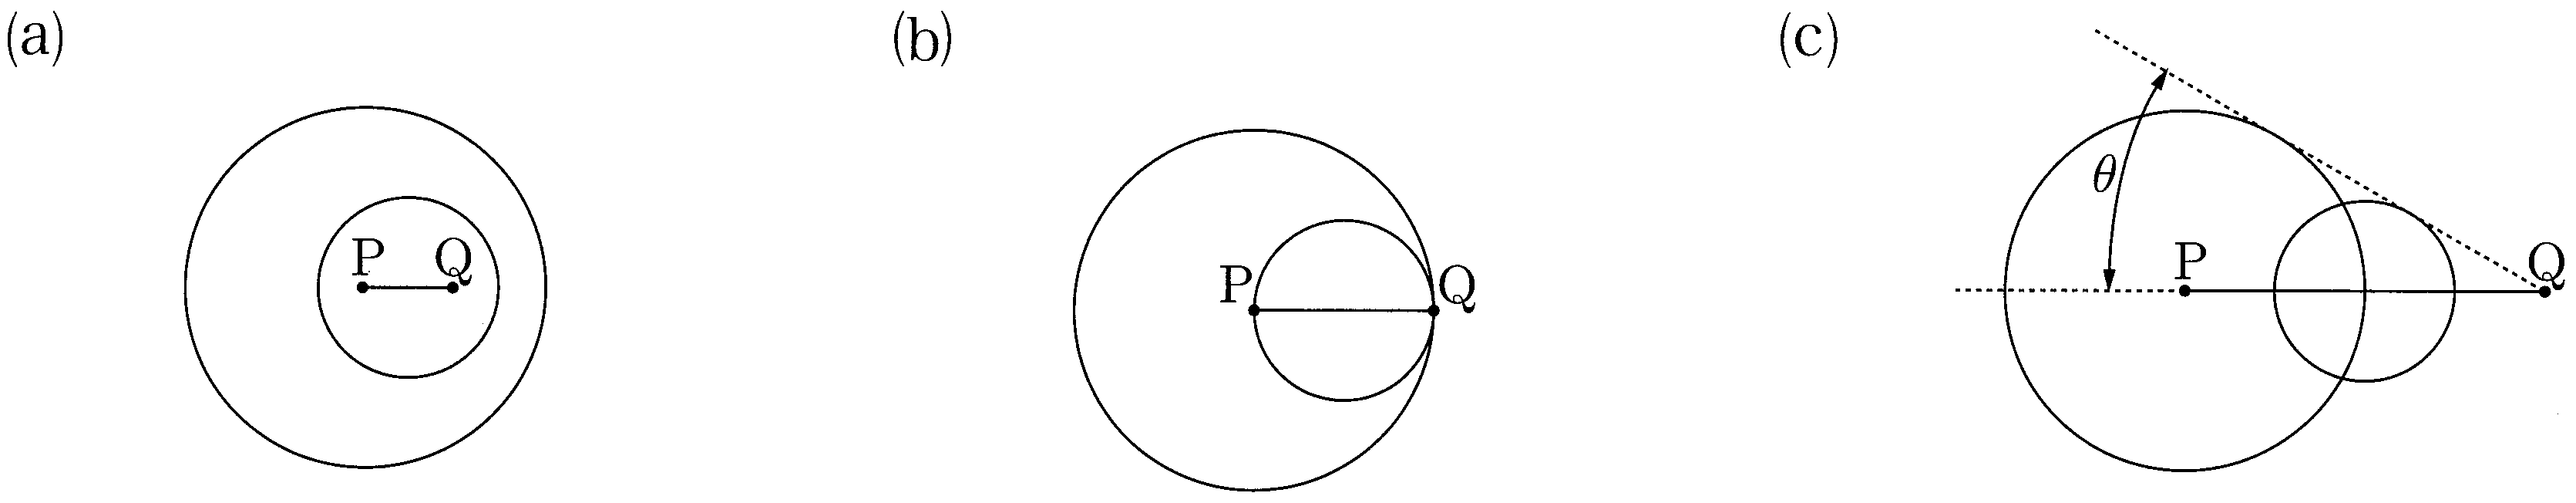
\includegraphics[keepaspectratio,width=150mm]{fig/n17_p42_wave.png}
\end{center}
\begin{komon}
\ko{1} このとき，図(a), (b), (c)に対応する$c$と$v$の関係を不等号を用いて表すと，\\
       \hspace*{3zw}(a)の場合，$c$\fbox{\MARU{1}}$v$\hspace{10mm}(b)の場合，$c$\fbox{\MARU{2}}$v$\hspace{10mm}(c)の場合，$c$\fbox{\MARU{3}}$v$
\ko{2} 図(c)の場合，角$\theta$を半頂角とする円錐の外部へは音は伝わることができない．この角$\theta$と$c,v$との関係式は，$\sin\theta=$\fbox{\MARU{4}}
\ko{3} 図(a)において$\mathrm{A}$の進行の向きに伝わる波長は\fbox{\MARU{5}}である．また，図(c)において$\mathrm{A}$の進行の向きと逆向きに伝わる波長は\fbox{\MARU{6}}である．
\end{komon}


\newpage

\KaiTitle{第17回　ドップラー効果と衝撃波}
\setlength{\columnseprule}{0.4pt}
\begin{multicols}{2}
\raggedcolumns

\Rank{A問題}
\MonN{29}{基本事項の確認}\par\nopagebreak
\begin{sisin}
ドップラー効果の公式を用いれば振動数は簡単に求められるであろうが，だからといって波源が動く場合と観測者が動く場合の両方を，単純に振動数が変わるだけだと考えるのは大きな誤りである．波源が動く場合には空間中を伝わる波の波長が変化し，観測者が動く場合には受け取る振動数が変化する．これらの変化を考える際には，式を当てはめる，という考え方ではなく，{\gtfamily ある瞬間と1秒後の図を描き，これを元に波の間隔や波の数を数える}，という方法で考えるように心がけて欲しい．

(4)の壁面の反射波は，\MARU{1}壁を観測者とみなす，\MARU{2}壁を音源とみなす，の2段階を経て振動数を求める．

(5)のように風が吹いている場合は，地面に対する音速が加速・減速したと考えて処理する．波長を求める際には，音速が変わったと考えるだけでよい．
\end{sisin}
\KaiHead
\begin{komon}
\ko{1} 音源が移動しているので前方では波の波長は圧縮され，
       \[\frac{340-20}{400}=0.8\U{m}\Ans\]
       また，後方への波の波長は伸びるので，
       \[\frac{340+20}{400}=0.9\U{m}\Ans\]
\ko{2} この音源から出ている波の波長は
       \[\lambda=\frac{340}{440}\U{m}\]
       遠ざかる観測者は，伝わってくる音波から逃げているので，1秒間に受け取る波は$340-10=330\U{m}$の区間に存在する波である．よって，その振動数は，
       \[\frac{330}{\lambda}=\frac{330}{340}\cdot440\fallingdotseq427.1\U{Hz}\Ans\]
       また，近づいてくる観測者が1秒間に受け取る波は$340+10=350\U{m}$の区間に存在する波である．よって，その振動数は，
       \[\frac{350}{\lambda}=\frac{350}{340}\cdot440\fallingdotseq452.9\U{Hz}\Ans\]
\ko{3} 前方では波の波長は圧縮される．(1)より，その波長は
       \[\lambda^\prime=\frac{340-20}{400}=\frac{4}{5}\U{m}\]
       この波長の音を観測者は近づきながら受け取るので，求める振動数は，
       \[\frac{340+10}{\lambda^\prime}=437.5\U{Hz}\Ans\]
       \begin{center}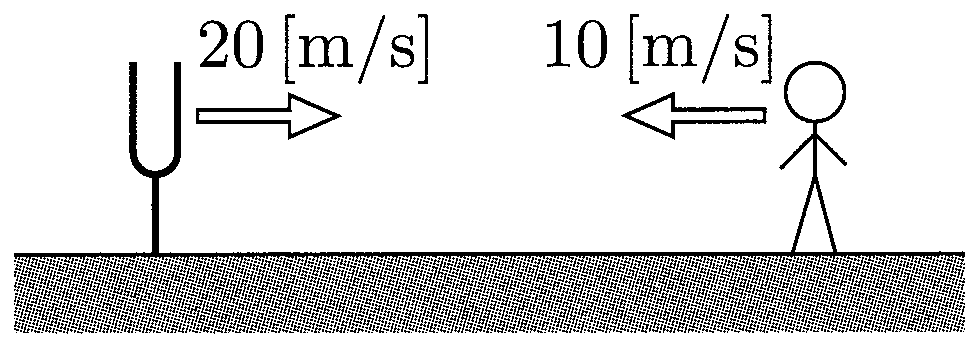
\includegraphics[keepaspectratio,width=62mm]{fig/n17_a29_z3.png}\end{center}
\ko{4} 位置関係は次図の通り．
       \begin{center}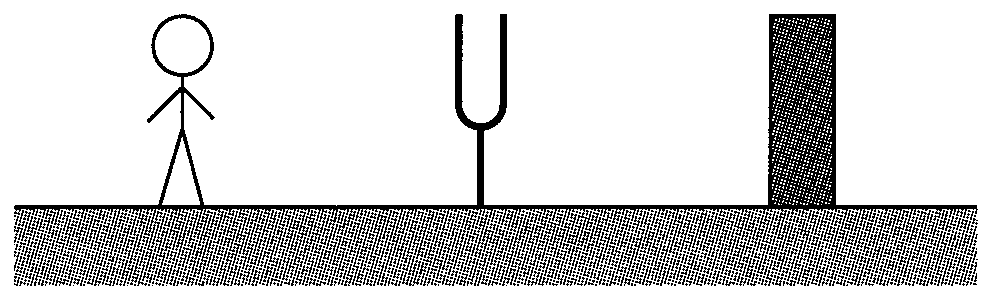
\includegraphics[keepaspectratio,width=62mm]{fig/n17_a29_z4.png}\end{center}
       直接音の振動数$f^\prime$は，
       \[f^\prime=\frac{340}{340+10}\cdot440\fallingdotseq427.4\U{Hz}\Ans\]
       壁面が受け取る音の振動数$f^{\prime\prime}$は，
       \[f^{\prime\prime}=\frac{340}{340-10}\cdot440\fallingdotseq453.3\U{Hz}\]
       であり，壁は移動していないので反射する音の振動数は$f^{\prime\prime}$のままとなる．よって，観測される反射音は，
       \[f^{\prime\prime}=453.3\U{Hz}\Ans\]
\ko{5} 音源の進行の向きへ音が伝わるときは追い風となるので地面に対する音速は$345\U{m/s}$となる．ゆえに進行方向へ出す音の波長$\lambda_1$は，
       \[\lambda_1=\frac{345-20}{400}\fallingdotseq0.81\U{m}\Ans\]
       また，音源の進行方向とは逆向きへ音が伝わるときは向かい風となるので地面に対する音速は$335\U{m/s}$となる．ゆえに後方へ出す音の波長$\lambda_2$は，
       \[\lambda_2=\frac{335+20}{400}\fallingdotseq0.89\U{m}\Ans\]
\end{komon}
% 誤植訂正（2026-09-05）：原本の解答は「地面に対する風速は345[m/s]」．風速ではなく音速．
\begin{bsHosoku}{参考}
(2)(3)では慣れてきたら公式を利用して求めればよい．
\end{bsHosoku}

\Rank{B問題}
\MonN{30}{音源が媒質に対して動く場合のドップラー効果}\par\nopagebreak
\begin{sisin}
問題の図に与えられたように波源が移動する場合，進行方向である$\mathrm{B}$側では波長が短くなり，進行方向の逆向きである$\mathrm{A}$側では波長が長くなる．そのため，$\mathrm{A}$, $\mathrm{B}$で静止している観測者（スピーカー）が受け取る振動数は異なる．$\mathrm{A}$が受け取った音は電気信号に変換されてスピーカーから同じ振動数を持つ音として出力されるので，$\mathrm{B}$にいる観測者は異なる振動数の音によるうなりを聞く．よって，音源の移動する速さを適当な文字で置き，$\mathrm{A}$, $\mathrm{B}$が受け取る振動数を計算し，その二つの振動数によるうなりを考えればよい．
\end{sisin}
\KaiHead
\hspace{1zw}音源の移動する速さを$v\U{m/s}$とおき，マイク$\mathrm{A}$および観測者$\mathrm{B}$が受ける音の振動数をそれぞれ$f_\mathrm{A}$, $f_\mathrm{B}\U{Hz}$とおく．
\[f_\mathrm{A}=\frac{340}{340+v}\times128\]
\[f_\mathrm{B}=\frac{340}{340-v}\times128\]
となる．これらはそれぞれ
\[f_\mathrm{A}=128\left(1+\frac{v}{340}\right)^{-1}\fallingdotseq128\left(1-\frac{v}{340}\right)\]
\[f_\mathrm{B}=128\left(1-\frac{v}{340}\right)^{-1}\fallingdotseq128\left(1+\frac{v}{340}\right)\]
と近似できるので，うなりの条件は，
\[f_\mathrm{B}-f_\mathrm{A}=128\cdot\frac{v}{340}\cdot2=2\]
これを解いて，
\[v=\frac{340}{128}\fallingdotseq2.66\U{m/s}\Ans\]

\MonN{31}{列車のドップラー効果}\par\nopagebreak
\begin{sisin}
マイクロホンで受けた音の振動数がある時刻を境に減少しているが，これは列車の警笛部分がマイクロホンの前を通過したためである．警笛がマイクロホンに接近してくるときには音は高く聞こえ（振動数が高くなり），警笛がマイクロホンから遠ざかるときには音は低く聞こえる（振動数が低くなる）．
\end{sisin}
\KaiHead
\begin{komon}
\ko{1} $t=t_\mathrm{A}$, $t_\mathrm{B}$で振動数が変化しているように観測されるのは，この時間に列車がマイクの前を通過するからである．
       \begin{center}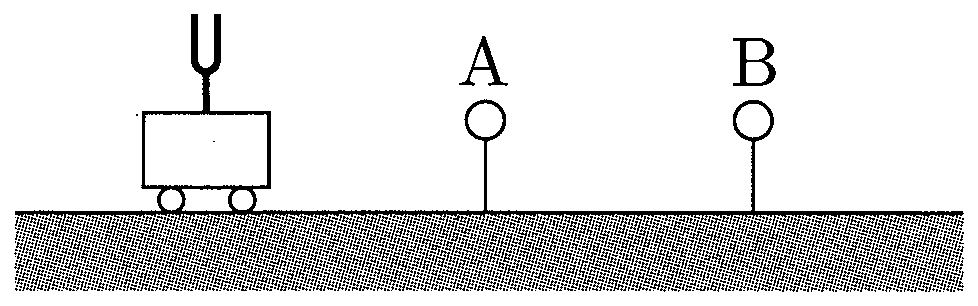
\includegraphics[keepaspectratio,width=62mm]{fig/n17_a31_train.png}\end{center}
       距離$40\U{m}$だけ離れたマイク$\mathrm{A}$, $\mathrm{B}$を通過するのに時間$t_\mathrm{B}-t_\mathrm{A}=8\U{s}$を要したのであるから，列車の速さは，
       \[v=\frac{40}{8}=5\U{m/s}\Ans\]
\ko{2} 警笛がマイクを通過する前については，
       \[f_1=\frac{340}{340-v}\times200\fallingdotseq203\U{Hz}\Ans\]
       警笛がマイクを通過した後については，
       \[f_2=\frac{340}{340+v}\times200\fallingdotseq197\U{Hz}\Ans\]
\end{komon}

\MonN[\Sitei]{32}{空間中に広がるドップラー効果}\par\nopagebreak
\begin{sisin}
波源が移動するときに空間中に広がる波面の様子を表した図である．波面に問題の図のような偏りが生じるのは，いったん波源から出た波は波源の移動によらず，{\gtfamily 波が出された位置を中心として円形状に広がっていく}ためである．

例えば次図のように波源が移動している場合，図の(a)の時点で出された波面は，（波源は右へ移動していくにもかかわらず）\MARU{1}点を中心にして(a)$\to$(b)$\to$(c)$\to$(d)の実線のように広がっていく．また，波源が移動して(b)の時点で出された波面は，\MARU{2}点を中心にして(b)$\to$(c)$\to$(d)の点線のように広がっていく．同様に，波源が移動して(c)の時点で出された波面は，\MARU{3}点を中心にして(c)$\to$(d)の点線のように広がっていく．
\begin{center}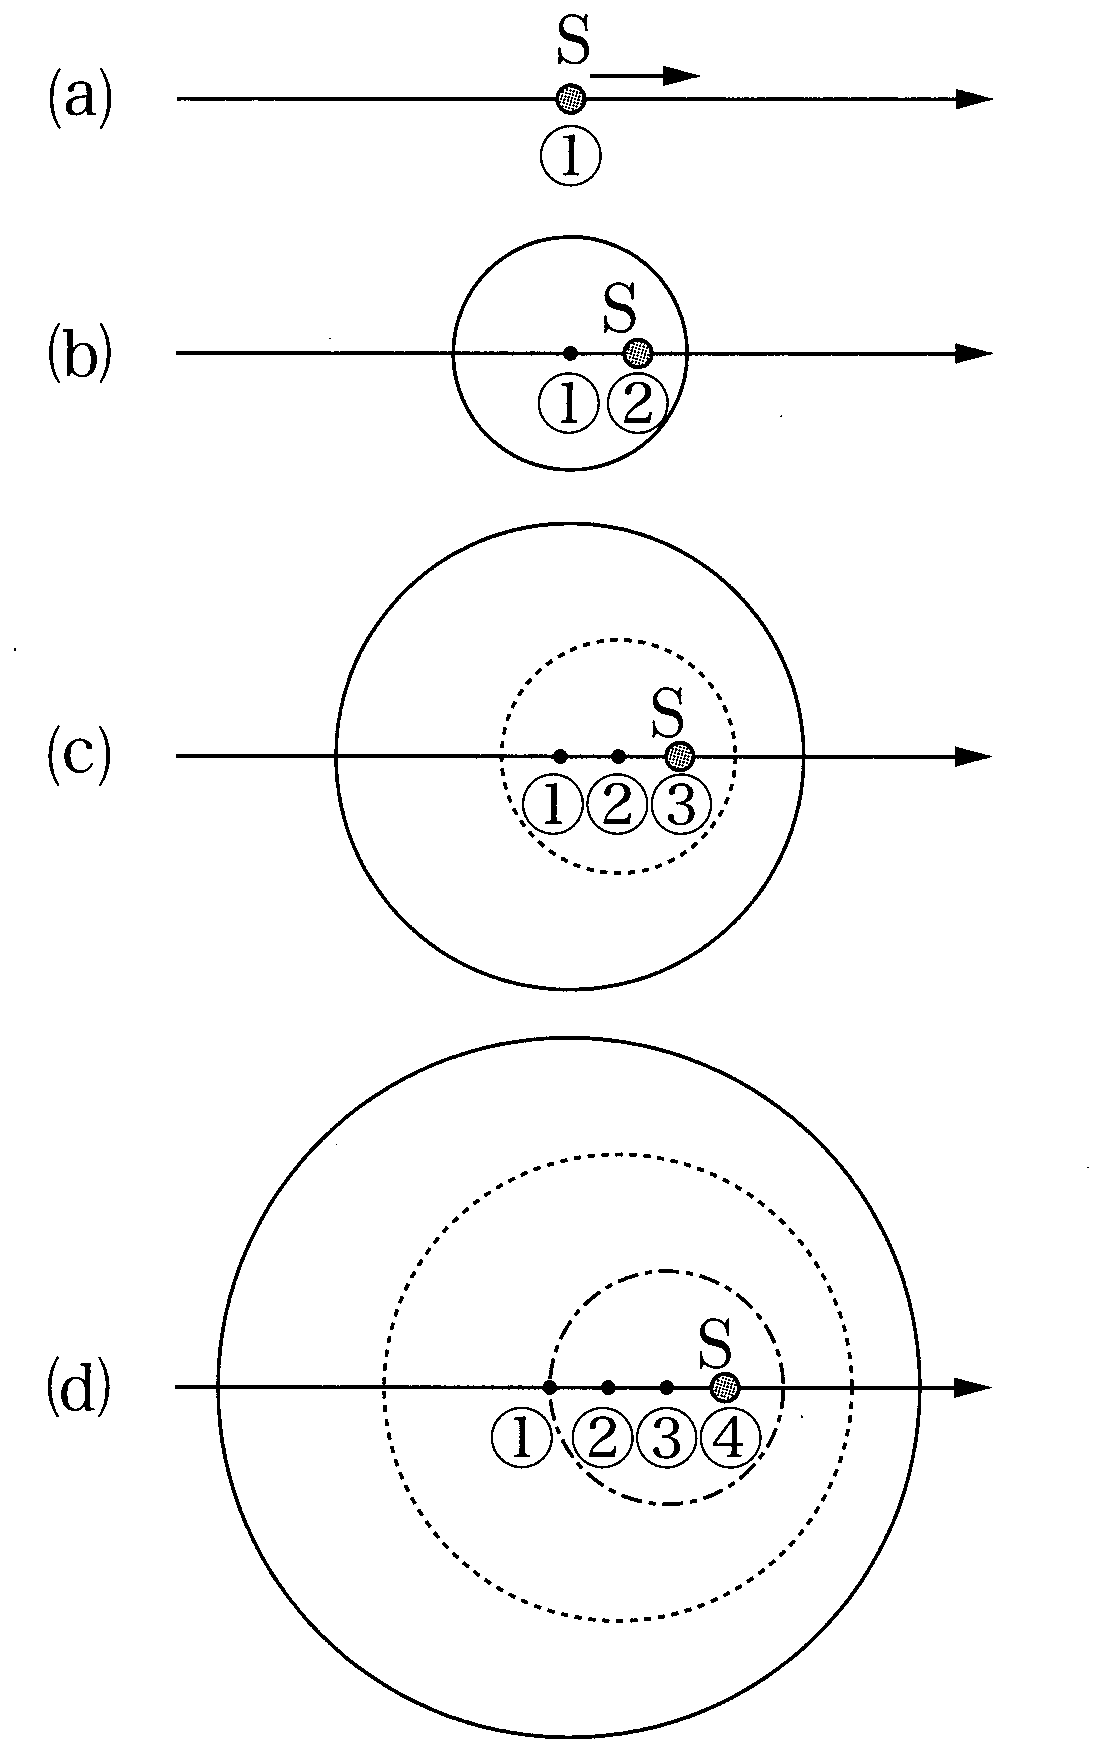
\includegraphics[keepaspectratio,width=48mm]{fig/n17_a32_sisin.png}\end{center}
このために偏った円状の波面が平面上に広がる．波源の進行方向では波面が詰まり，波源の進行方向の逆側では波面が間延びする．

波源の進行直線上での波長変化や観測される振動数の変化は前問までと同様にして考えればよい．
\end{sisin}
\KaiHead
\begin{komon}
\ko{1} 波源$\mathrm{A}$の西側の波面が詰まり，東側の波面が伸びているので，この波源は西向きに進んでいる．\hspace*{\fill}\Ans
\ko{2} $\mathrm{A}$から東に向かう波とは，波源の進行方向とは逆向きに出された波のことであるから，その波長は，
       \[\lambda_1=\frac{V+v}{f}\U{m}\Ans\]
\ko{3} $\mathrm{B}$が静止している場合には，波長$\lambda_1=\dfrac{V+v}{f}$の波が伝わってくるから，$\mathrm{B}$で観測される振動数$f_1$は，
       \[f_1=\frac{V}{\lambda_1}=\frac{V}{V+v}f\U{Hz}\Ans\]
       \begin{center}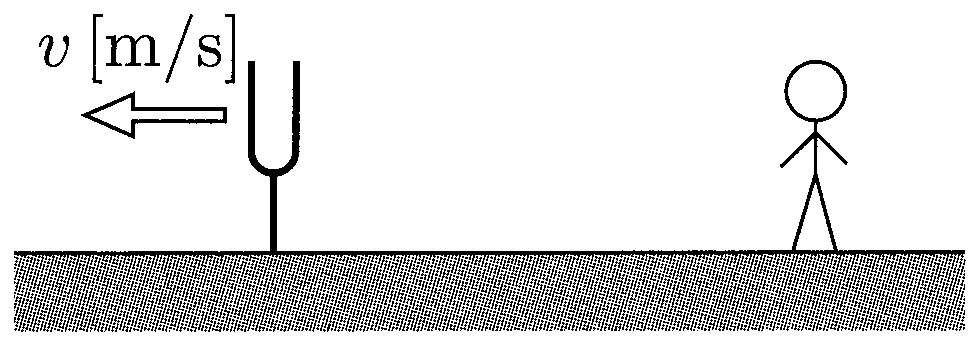
\includegraphics[keepaspectratio,width=62mm]{fig/n17_a32_z2.png}\end{center}
\ko{4} $\mathrm{B}$が速さ$u\U{m/s}$で西向きに移動しており，波長$\lambda_1=\dfrac{V+v}{f}$の波の中を波源に近づいているので，求める振動数$f_2$は，
       \[f_2=\frac{V+u}{\lambda_1}=\frac{V+u}{V+v}f\U{Hz}\Ans\]
       \begin{center}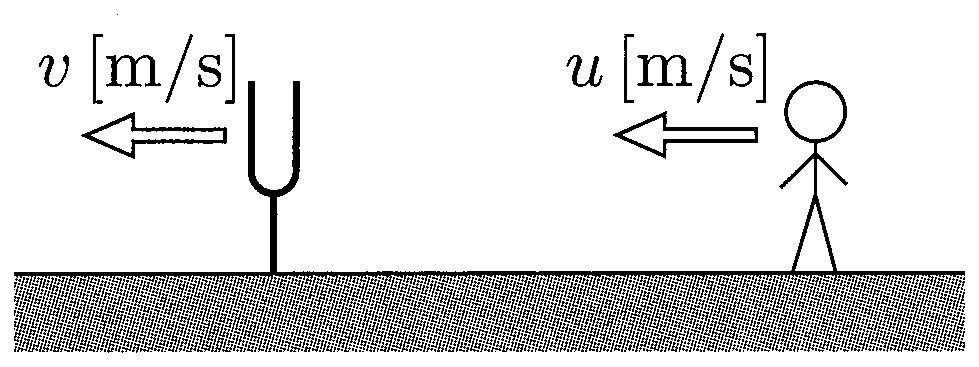
\includegraphics[keepaspectratio,width=62mm]{fig/n17_a32_z4.png}\end{center}
\end{komon}

\MonN{33}{一直線上のドップラー効果}\par\nopagebreak
\begin{sisin}
本問の場合には与えられていない値が非常に多いので，超特急が追い越していく前と後について適当な図を描き，必要と思われるものについては文字を置き，式を立てて考えていこう．
\end{sisin}
\KaiHead
\begin{komon}
\ko{1} 超特急の速さを$V\U{km/h}$とし，超特急の警笛の振動数を$f_0\U{Hz}$とする．超特急が自動車の前方からやってきている最中と，後方に去っていく最中の位置・速度の関係を図示すると次図のようになる．
       \begin{center}前方からやってきている最中\\ 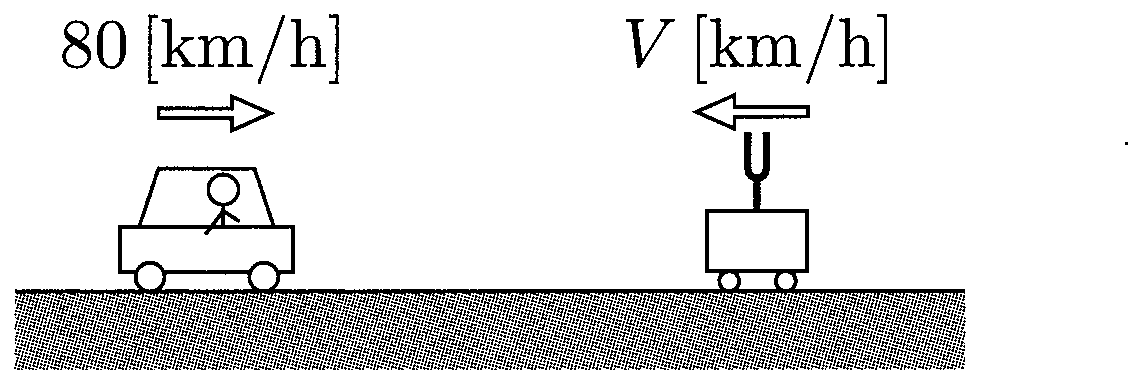
\includegraphics[keepaspectratio,width=62mm]{fig/n17_a33_z1.png}\\[2mm] 後方に去っていく最中\\ 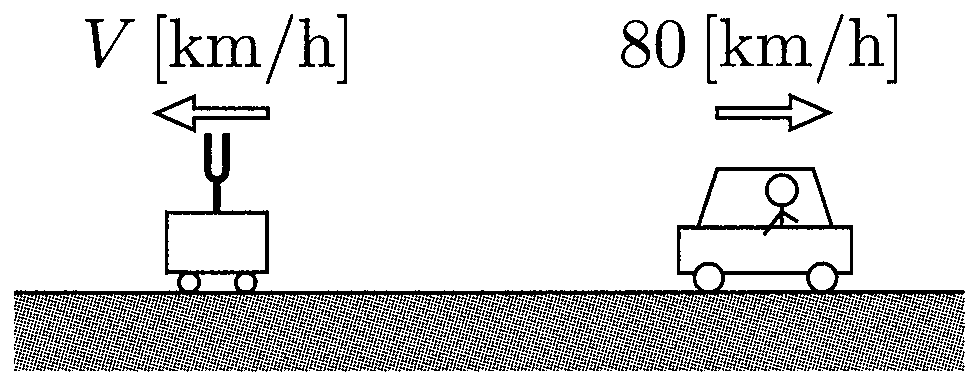
\includegraphics[keepaspectratio,width=62mm]{fig/n17_a33_z2.png}\end{center}
       音源，観測者共に移動しているドップラー効果であるから，前方からやってきている最中に観測者が聞く音の振動数は，
       \[f_1=\frac{1200+80}{1200-V}f_0\U{Hz}\]
       また，後方に去っていく最中に観測者が聞く音の振動数は，
       \[f_2=\frac{1200-80}{1200+V}f_0\U{Hz}\]
       である．この二つの振動数の比が$\dfrac{8}{5}$であるから，$f_1>f_2$に注意して，
       \[\frac{f_1}{f_2}=\frac{1200+V}{1200-V}\cdot\frac{1200+80}{1200-80}=\frac{8}{5}\]
       これを解いて，
       \[V=200\U{km/h}\Ans\]
\ko{2} 止まっている人が警笛を聞く場合には次図のような位置・速度関係になる．
       \begin{center}前方からやってきている最中\\ 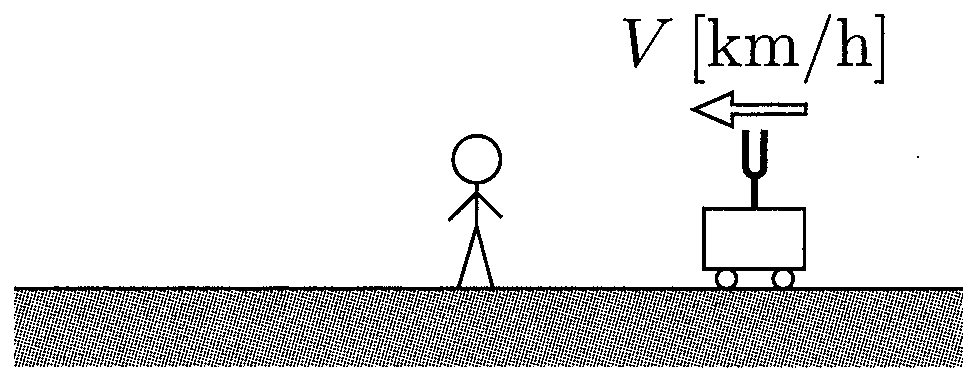
\includegraphics[keepaspectratio,width=62mm]{fig/n17_a33_z3.png}\\[2mm] 後方に去っていく最中\\ 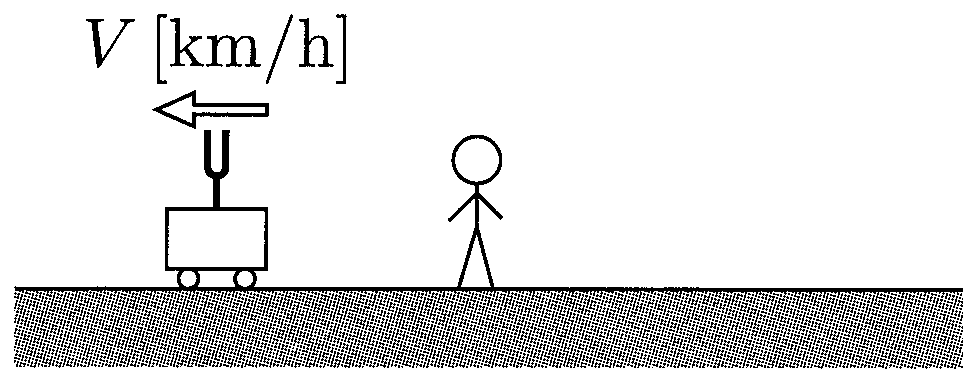
\includegraphics[keepaspectratio,width=62mm]{fig/n17_a33_z4.png}\end{center}
       ゆえに，それぞれの時に観測される振動数は，
       \[f_1^\prime=\frac{1200}{1200-V}f_0\U{Hz}\]
       \[f_2^\prime=\frac{1200}{1200+V}f_0\U{Hz}\]
       である．よってこの二つの振動数の比を取ると，
       \[\frac{f_1^\prime}{f_2^\prime}=\frac{1200+V}{1200-V}=\frac{7}{5}\Ans\]
\end{komon}

\MonN{34}{ドップラー効果とうなり}\par\nopagebreak
\begin{sisin}
うなりが$N\U{Hz}$であることから$\mathrm{B}$のスピーカーの振動数を決めるが，この条件だけでは$\mathrm{B}$の振動数が，$f+N\U{Hz}$, $f-N\U{Hz}$のどちらであるかを決定することができない．それを決めるのが「遠ざけたときにうなりがなくなった」という条件である．ドップラー効果により，{\gtfamily 遠ざけるときには観測される振動数は小さくなる}，とわかるから，$\mathrm{B}$の振動数がどちらであるのかを決定できる．

(3)では，まず$\mathrm{A}$, $\mathrm{B}$のもともとの振動数の大小関係に着目し，観測者がどちら向きに動けば，$\mathrm{A}$, $\mathrm{B}$の音が同一振動数として聞こえるようになりうるのかを考えるところから取りかかること．
\end{sisin}
\KaiHead
\begin{komon}
\ko{1} 音源$\mathrm{B}$を遠ざけるとき，音源$\mathrm{B}$からの音を観測者が聞くときの振動数は$f^\prime$に比べて小さくなる．$\mathrm{B}$をある一定の速さで遠ざけたところ，$\mathrm{B}$からやってくる音の振動数が$f\U{Hz}$の音として観測されてうなりがなくなるというのだから，音源$\mathrm{B}$の振動数$f^\prime\U{Hz}$は$f\U{Hz}$よりも大きいことが分かる．

       音源$\mathrm{B}$が動いていないときには，観測者$\mathrm{O}$が観測する音は音源$\mathrm{A}$, $\mathrm{B}$の振動数と同じであり，この二つの音によるうなりが$N$回であったから，
       \[|f^\prime-f|=N\]
       である．$f^\prime>f$であることに注意してこれを解くと，
       \[f^\prime=f+N\U{Hz}\Ans\]
\ko{2} $\mathrm{B}$を速さ$v\U{m/s}$で遠ざけるとき，観測者$\mathrm{O}$が聞く音の振動数は，音源移動のドップラー効果なので，
       \[f^{\prime\prime}=\frac{c}{c+v}f^\prime\U{Hz}\]
       このとき，うなりがなくなったので，
       \[f^{\prime\prime}=f\]
       である．これを解いて$v\U{m/s}$を求めると，
       \[v=\frac{N}{f}c\U{m/s}\Ans\]
\ko{3} 音源の振動数は$\mathrm{B}$の方が大きい．観測者が波源に近づくときは音の振動数が高く聞こえるので，$\mathrm{A}$, $\mathrm{B}$から聞こえる音の振動数が一致するためには，観測者$\mathrm{O}$は$\mathrm{A}$の方に近づかなければならないと言える．（$\mathrm{B}$に近づくと，$\mathrm{B}$から聞こえる音の振動数がさらに大きくなり，また$\mathrm{A}$から聞こえる音の振動数はさらに小さくなるので，同じ値になることは決してない）

       $\mathrm{O}$が$\mathrm{A}$に近づく速さを$u\U{m/s}$として，$\mathrm{O}$が聞く振動数を求めると，観測者移動のドップラー効果であるから，
       \begin{center}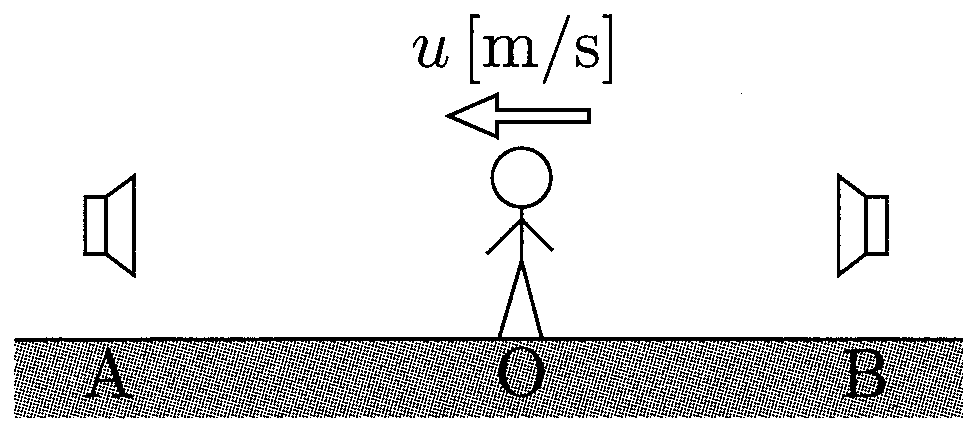
\includegraphics[keepaspectratio,width=52mm]{fig/n17_a34_aob.png}\end{center}
       \[f_\mathrm{A}=\frac{c+u}{c}f\U{Hz}\]
       \[f_\mathrm{B}=\frac{c-u}{c}f^\prime\U{Hz}\]
       この二つの振動数が一致したとき，うなりが観測されなくなるので，
       \[\frac{c+u}{c}f=\frac{c-u}{c}f^\prime\]
       これを解いて，
       \[u=\frac{N}{2f+N}c\U{m/s}\]
       である．よって，うなりが観測されなくなるときの$\mathrm{O}$の速度は，
       \[\mathrm{A}\text{に向かって速さ}\ \frac{N}{2f+N}c\U{m/s}\Ans\]
\end{komon}

\MonN[\Sitei]{35}{反射波によるドップラー効果および風の効果}\par\nopagebreak
\begin{sisin}
音が右向きに進む場合と左向きに進む場合とで音速が異なることに注意．音波が右向きに進む場合には追い風となって加速されるが，音波が左向きに進む場合には向かい風となって減速される．
\end{sisin}
\KaiHead
\begin{komon}
\ko{1} 音源$\mathrm{S}$から観測者$\mathrm{O}$に向かって直接音が左向きに進むときには風が向かい風となるため，音速は$c-w\U{m/s}$に減速される．観測者移動のドップラー効果であるから，直接音の振動数$f_1$は，
       \[f_1=\frac{(c-w)+u}{c-w}f\U{Hz}\Ans\]
\ko{2} 音源$\mathrm{S}$から壁$\mathrm{R}$へ音が向かって右向きに進むときには風が追い風となるので，音速は$c+w\U{m/s}$となる．壁$\mathrm{R}$が受け取る振動数は，(1)と同様に考えて，
       \[f^\prime=\frac{(c+w)+V}{c+w}f\U{Hz}\]
       また，壁$\mathrm{R}$で反射した音が観測者に向かって左向きに進むときには風が向かい風となるため，音速は$c-w\U{m/s}$に減速される．よって，壁$\mathrm{R}$からの反射音を観測者が聞いたときの振動数$f_2$は，壁$\mathrm{R}$を振動数$f^\prime\U{Hz}$の音源としたドップラー効果と考えて，
       \[f_2=\frac{(c-w)+u}{(c-w)-V}f^\prime\U{Hz}\]
       以上より，
       \[f_2=\frac{(c-w+u)(c+w+V)}{(c-w-V)(c+w)}f\U{Hz}\Ans\]
\end{komon}

\MonN{36}{直接音と反射音によるうなり}\par\nopagebreak
\begin{sisin}
マイクロホンのキャッチした音が，ある時間間隔ごとに強から弱を経て強となる変化を繰り返す，すなわち「うなり」を観測するのは，振動数がわずかに異なる二つの音を観測するためである．直接音，反射音の振動数を求めて，うなりを計算すればよい．

時間間隔$t_1\U{s}$ごとに強から弱を経て強となる変化を聞いたということは，$1\U{s}$間にうなりを$\dfrac{1}{t_1}$回だけ観測していることを意味する．
\end{sisin}
\KaiHead
\begin{komon}
\ko{1} 実験\MARU{1}において，スピーカー$\mathrm{S}$からマイクロホン$\mathrm{M}$にやってくる直接音の振動数は，
       \[f_1=\frac{c-v}{c}f_0\U{Hz}\]
       スピーカー$\mathrm{S}$から反射壁$\mathrm{R}$にやってくる音の振動数は
       \[f^\prime=\frac{c}{c}f_0\U{Hz}\]
       であり，$\mathrm{R}$で反射してマイクロホン$\mathrm{M}$に向かう反射音の振動数は，
       \[f_2=\frac{c+v}{c}f^\prime=\frac{c+v}{c}f_0\U{Hz}\]
       マイクロホン$\mathrm{M}$ではこの二つの音によるうなりが観測される．$1\U{s}$間にうなりを$\dfrac{1}{t_1}$回だけ観測しているので，
       \[|f_2-f_1|=\frac{2v}{c}f_0=\frac{1}{t_1}\]
       が成立する．よってこれを解いて，
       \[c=2vt_1f_0\U{m/s}\Ans\]
\ko{2} 実験\MARU{2}において，スピーカー$\mathrm{S}$からマイクロホン$\mathrm{M}$にやってくる直接音の振動数は，
       \[f_3=\frac{c-u}{c-u}f_0\U{Hz}\]
       スピーカー$\mathrm{S}$から反射壁$\mathrm{R}$にやってくる音の振動数は
       \[f^{\prime\prime}=\frac{c}{c-u}f_0\U{Hz}\]
       であり，$\mathrm{R}$で反射してマイクロホン$\mathrm{M}$に向かう反射音の振動数は，
       \[f_4=\frac{c+u}{c}f^{\prime\prime}=\frac{c+u}{c-u}f_0\U{Hz}\]
       マイクロホン$\mathrm{M}$ではこの二つの音によるうなりが観測される．$1\U{s}$間にうなりを$\dfrac{1}{t_2}$回だけ観測しているので，
       \[|f_4-f_3|=\frac{2u}{c-u}f_0=\frac{1}{t_2}\]
       が成立する．これに(1)を代入して解くと，
       \[t_2=\frac{2vt_1f_0-u}{2uf_0}\U{s}\Ans\]
\end{komon}
\begin{bsHosoku}{別解}
少し難しい考え方だが，以下のように考えて解くことも可能である．

まず(1)では，$\mathrm{S}$, $\mathrm{R}$が静止しているため，マイクロホン$\mathrm{M}$を通過して右向きに進行する波，およびマイクロホン$\mathrm{M}$を通過して左向きに進行する波はいずれも同一波長で，$\lambda_1=\dfrac{c}{f_0}\U{m}$である．ゆえにこの空間には同一波長の右向きの波，左向きの波が重なることにより定在波が生じており，腹や節が$\dfrac{\lambda_1}{2}\U{m}$の等間隔で並んでいる．この空間を$\mathrm{M}$が右向きに進んでいくときに，腹を通過したときには音が大きく，また節を通過したときには音が小さくなるから，「$t_1\U{s}$ごとに強から弱を経て強となる変化を繰り返した」とは，速さ$v\U{m/s}$で右に進むときに$t_1\U{s}$ごとに腹を通過したことを意味する．よって，
\[v\cdot t_1=\frac{\lambda_1}{2}\]
が成立し，これより
\[c=2vt_1f_0\U{m/s}\]

一方，(2)の場合には，$\mathrm{S}$は右向きに速さ$u\U{m/s}$で移動しているので，$\mathrm{S}$から右向きに波長が
\[\lambda_2=\frac{c-u}{f_0}\U{m}\]
に圧縮された波が出されている．$\mathrm{R}$は固定されているから，$\mathrm{R}$で反射して左向きに進む波の波長も$\lambda_2\U{m}$になる．以上より，この空間には波長$\lambda_2\U{m}$の波による定在波が出来ており，腹や節が$\dfrac{\lambda_2}{2}\U{m}$の等間隔で並んでいる．(1)の場合と同様に考えると，
\[u\cdot t_2=\frac{\lambda_2}{2}\]
が成立し，これを解いて，
\[t_2=\frac{2vt_1f_0-u}{2uf_0}\U{s}\]
が導かれる．
\end{bsHosoku}

\MonN[\Sitei]{37}{斜めドップラー効果}\par\nopagebreak
\begin{sisin}
音源が運動する直線上に観測者がいない場合には，音源と観測者を直線で結び，この直線方向の速度成分を取り出してドップラー効果を考える．

音源が$\mathrm{X}$の無限遠方にいるときには図中の$\theta$が$0^\circ$の場合に，また音源が$\mathrm{Y}$の無限遠方にいるときには$\theta$が$180^\circ$の場合に対応する．
\end{sisin}
\KaiHead
\begin{komon}
\ko{1} 音源$\mathrm{S}$の速度ベクトルの$\mathrm{AB}$直線方向成分は$v\cos\theta\U{m/s}$である．すなわち，$\mathrm{B}$からやってくる音のドップラー効果は，音源が観測者に向かって速さ$v\cos\theta\U{m/s}$で近づくと考えて式を立てればよい．ゆえに，
       \[f^\prime=\frac{c}{c-v\cos\theta}f_0\U{Hz}\Ans\]
\ko{2} $\mathrm{S}$が$\mathrm{X}$の無限遠方にあるときとは，(1)の$\mathrm{B}$点が$\theta\to0^\circ$の極限に近づいたときだとみなせる．よって，$\mathrm{X}$の無限遠方から音が聞こえ始めたときの振動数は，(1)式の極限を取って，
       \[f_1=\lim_{\theta\to0^\circ}f^\prime=\frac{c}{c-v}f_0\U{Hz}\]
       また，$\mathrm{S}$が$\mathrm{Y}$の無限遠方にあるときとは，(1)の$\mathrm{B}$点が$\theta\to180^\circ$の極限に近づいたときだとみなせる．よって，$\mathrm{Y}$の無限遠方から音が聞こえてくるときの振動数は，(1)式の極限を取って，
       \[f_2=\lim_{\theta\to180^\circ}f^\prime=\frac{c}{c+v}f_0\U{Hz}\]
       題意より，
       \[\frac{f_2}{f_1}=\frac{c-v}{c+v}=\frac{1}{3}\]
       これを解いて，
       \[v=\frac{1}{2}c\U{m/s}\Ans\]
\end{komon}

\MonN{38}{斜めドップラー効果と音の伝わる速さ}\par\nopagebreak
\begin{sisin}
(2)に注意．音源から観測者までは距離があるので，音源で出された音がすぐさま$\mathrm{P}$にいる観測者に届くわけではない．出されてから$\mathrm{P}$に届くまでの時間を考えよ．
\end{sisin}
\KaiHead
\begin{komon}
\ko{1} 車を文字$\mathrm{S}$で表す．$\mathrm{P}$と車$\mathrm{S}$とを結ぶ直線を作図し，これと車$\mathrm{S}$の速度ベクトルのなす角度を$\varphi$とする．
       \begin{center}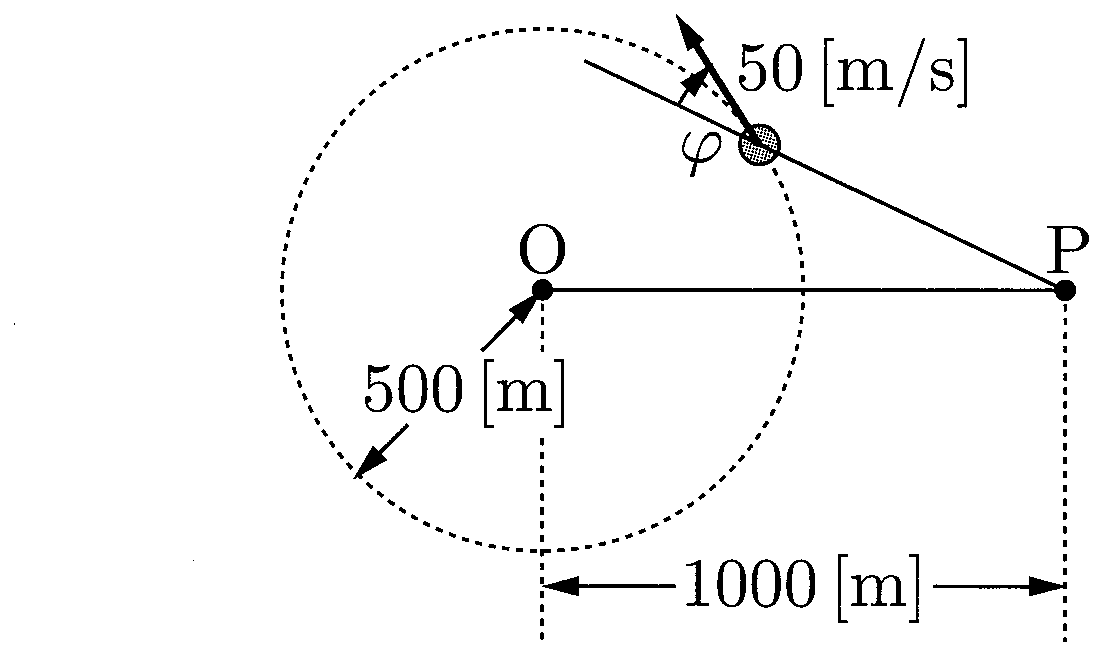
\includegraphics[keepaspectratio,width=62mm]{fig/n17_a38_z1.png}\end{center}
       車がこの円軌道を一周するときに，この図のように取った角度$\varphi$は$-180^\circ\leqq\varphi\leqq180^\circ$の範囲で変化する．上図のような位置から車$\mathrm{S}$が発した音は，$\mathrm{P}$点に向かって直線的にやってきて，ドップラー効果により振動数が
       \[f=\frac{350}{350+50\cos\varphi}\cdot400\U{Hz}\]
       の音として観測される．よって，$-180^\circ\leqq\varphi\leqq180^\circ$の範囲でこの最大値・最小値を取ると，観測者の聞く音の振動数の最大値は$\varphi=180^\circ$のときで，
       \[f_{\max}=\frac{350}{350-50}\cdot400\fallingdotseq467\U{Hz}\Ans\]
       また，観測者の聞く音の振動数の最小値は$\varphi=0^\circ$のときで，
       \[f_{\min}=\frac{350}{350+50}\cdot400=350\U{Hz}\Ans\]
\ko{2} まず，$400\U{Hz}$の爆音が円軌道のどの点から出されたものかを考える．$400\U{Hz}$とは音源$\mathrm{S}$の爆音の振動数そのものであるから，この爆音は，観測者と音源とを結ぶ方向の速度成分が存在しないような点，すなわち図の$\mathrm{A}$点（$\varphi=90^\circ$の点）もしくは$\mathrm{B}$点（$\varphi=-90^\circ$の点）のいずれかから出された音であると分かる．
       \begin{center}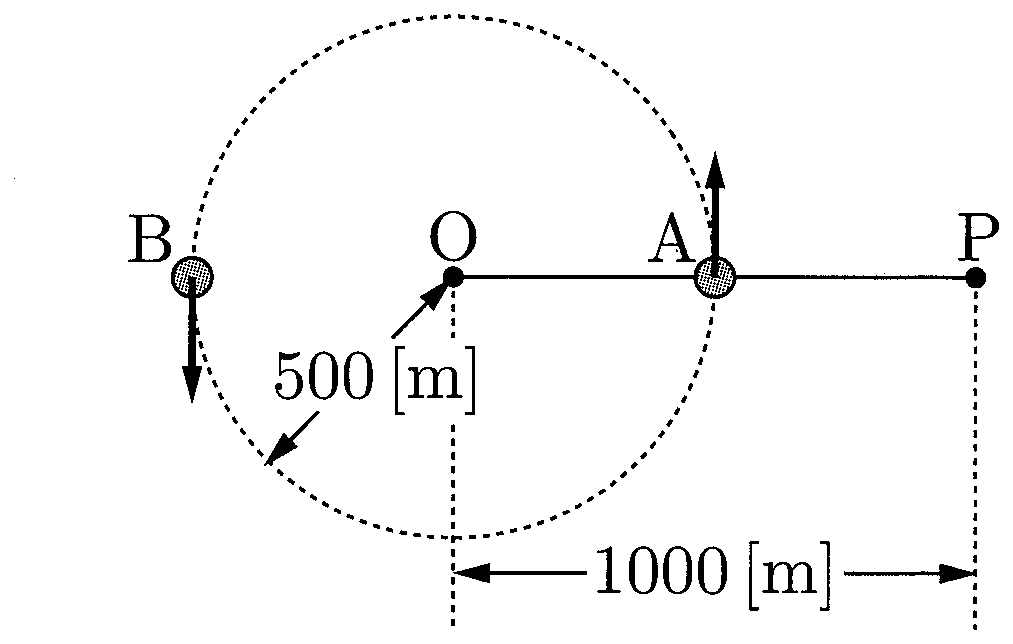
\includegraphics[keepaspectratio,width=62mm]{fig/n17_a38_z2.png}\end{center}
       $\mathrm{A}$点から$\mathrm{B}$点へこの音源$\mathrm{S}$が進む場合には，車$\mathrm{S}$と$\mathrm{P}$とを結ぶ直線方向の速度成分が，$\overrightarrow{\mathrm{PS}}$の向きに大きくなるため，車から聞こえてくる音の振動数は徐々に小さくなる（角度$\varphi$が$\varphi=90^\circ$から減少していくため，(1)の式より振動数は$\varphi=0^\circ$となるまで単調減少していく）．

       一方，$\mathrm{B}$点から$\mathrm{A}$点へ$\mathrm{S}$が進む場合には，車$\mathrm{S}$と$\mathrm{P}$とを結ぶ直線方向の速度成分が，$\overrightarrow{\mathrm{SP}}$の向きに大きくなるため，車から聞こえてくる音の振動数は徐々に大きくなる．

       ゆえに，題意にある$400\U{Hz}$の爆音とは，上図の$\mathrm{A}$で出された爆音であると分かる．車がこの$\mathrm{A}$点を通過した時刻を$t=0\U{s}$とすると，$\mathrm{AP}$間の距離が$500\U{m}$であるから，$\mathrm{P}$点にいる観測者が$400\U{Hz}$の爆音を聞く時刻は，
       \[t_\mathrm{A}=\frac{500}{350}\fallingdotseq1.43\U{s}\]
       である．

       また，爆音が最小の振動数に聞こえるのは，速度ベクトルが音源$\mathrm{S}$と観測者を結ぶ直線方向を向き，かつ遠ざかる向きとなる$\varphi=0^\circ$の点，すなわち次図の$\mathrm{C}$点から爆音が出されたときである．
       \begin{center}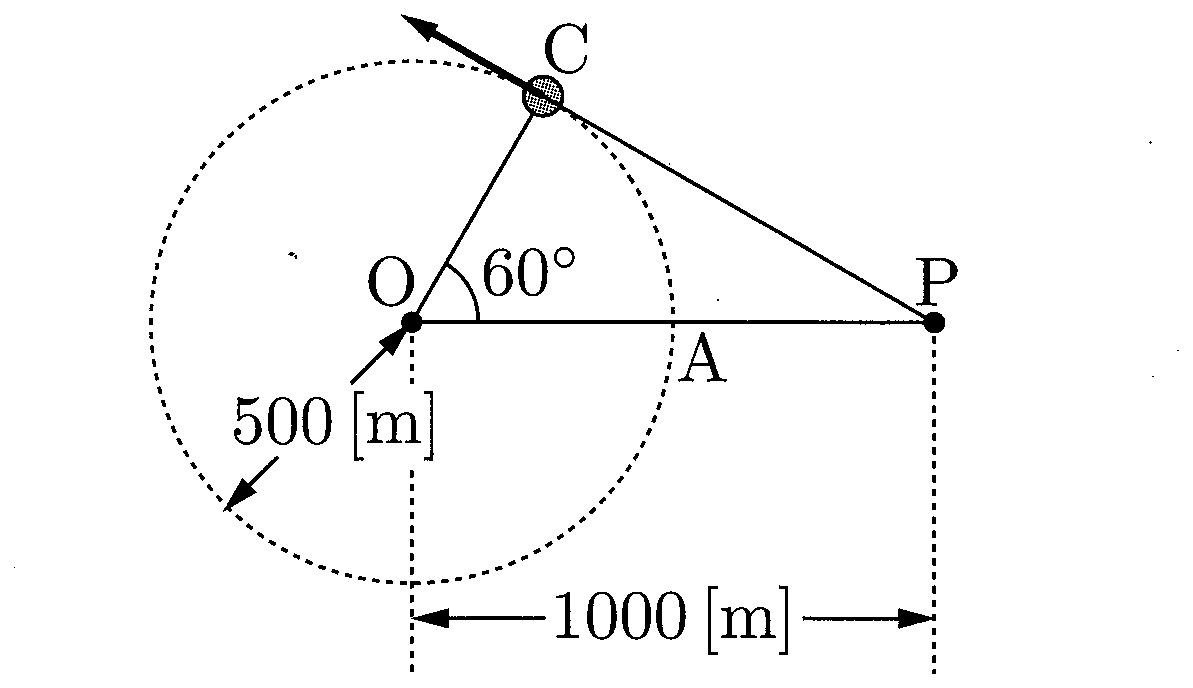
\includegraphics[keepaspectratio,width=62mm]{fig/n17_a38_z3.png}\end{center}
       この$\mathrm{C}$点は，図の幾何学的関係より$\angle\mathrm{AOC}=60^\circ$の点に対応する．まず，車が$\mathrm{A}$点から$\mathrm{C}$点に移動するのに
       \[\frac{2\pi\times500}{50}\times\frac{60^\circ}{360^\circ}\fallingdotseq10.47\U{s}\]
       を要し，そしてこの$\mathrm{C}$点から$\mathrm{P}$点に向かって距離$500\sqrt{3}\U{m}$だけ音が進んで観測者が$f_{\min}$の振動数の爆音を観測することになるので，観測者が$f_{\min}$の振動数の爆音を観測する時刻は，
       \[t_\mathrm{C}=10.47+\frac{500\sqrt{3}}{350}\fallingdotseq12.94\U{s}\]
       である．よって，$400\U{Hz}$の爆音を聞いてから最小の振動数の音を聞くまでに要した時間は，
       \[t_\mathrm{C}-t_\mathrm{A}=12.94-1.43=11.51\U{s}\Ans\]
\end{komon}

\Rank{C問題}
\MonN{39}{ドップラー効果}\par\nopagebreak
\begin{sisin}
基本的な指針は今までの問題と全く同一で，各状態の図を描き，ドップラー効果を考えていけばよい．与えられていない物理量は文字で置いた上で式を立てていこう．
\end{sisin}
\KaiHead
\begin{komon}
\ko{1} 救急車のサイレン音を$f_0\U{Hz}$，速さを$V\U{m/s}$とし，車を止めながら救急車が追い越していく様子を図示すると次図のようになる．
       \begin{center}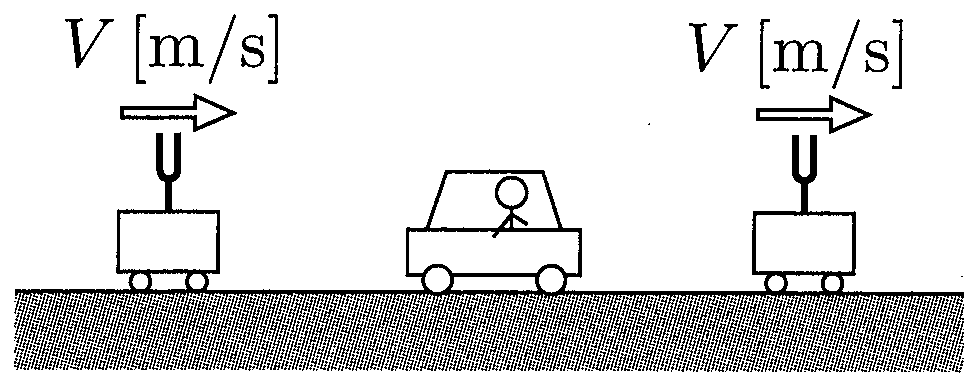
\includegraphics[keepaspectratio,width=62mm]{fig/n17_a39_z1.png}\end{center}
       救急車のサイレン音は$1260\U{Hz}$から$1092\U{Hz}$へと変化したので，各々のときのドップラー効果についての式を立てると，
       \[1260=\frac{336}{336-V}f_0\]
       \[1092=\frac{336}{336+V}f_0\]
       が成立する．この2式を連立させて$f_0$, $V$を得る．まず2式の比を取って$f_0$を消すと，
       \[\frac{1260}{1092}=\frac{336+V}{336-V}\]
       であるから，これを解いて，
       \[V=24\U{m/s}\Ans\]
       またこれを上式に代入して，
       \[f_0=1170\U{Hz}\Ans\]
\ko{2} 追い越す前については，観測者に向かってやってくる波は，波源が進行方向に出している波であるから波長は圧縮されており，
       \[\lambda_1=\frac{336-24}{1170}\fallingdotseq0.267\U{m}\Ans\]
       また追い越した後については，観測者に向かってやってくる波は，波源が進行方向と逆向きに出している波であるから波長は伸長されており，
       \[\lambda_2=\frac{336+24}{1170}\fallingdotseq0.308\U{m}\Ans\]
\ko{3} このときの位置・速度の関係は次図のようである．
       \begin{center}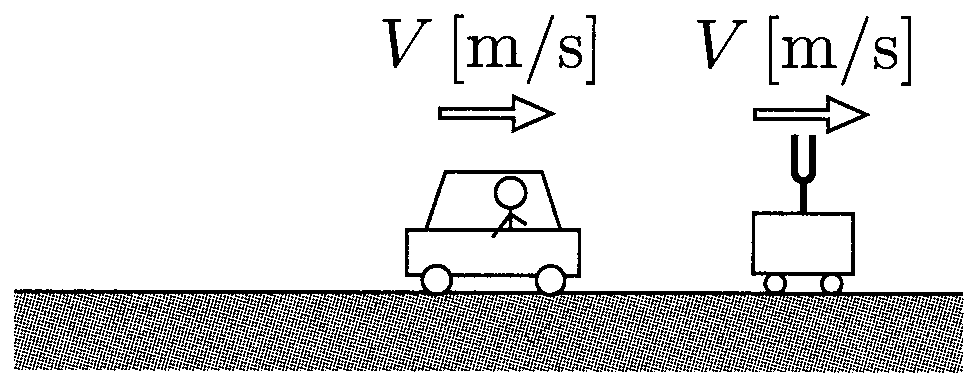
\includegraphics[keepaspectratio,width=62mm]{fig/n17_a39_z3.png}\end{center}
       音源，観測者共に移動するドップラー効果であるから，観測者の聞く振動数は，
       \[f_1=\frac{336+V}{336+V}\cdot1170=1170\U{Hz}\Ans\]
\ko{4} 波源が出す波の波長は，観測者の移動によっては変化せず，波源がどのように移動しているのかによってのみ決まる．追い越し前・後のいずれでも波源は静止しているので，サイレン音の波長は変わらず，
       \[\lambda_3=\frac{336}{1170}\fallingdotseq0.287\U{m}\Ans\]
\ko{5} 救急車が静止していて，観測者の車がこれを追い越して走行している場合に観測者の聞くサイレンの音の振動数は，
       \begin{center}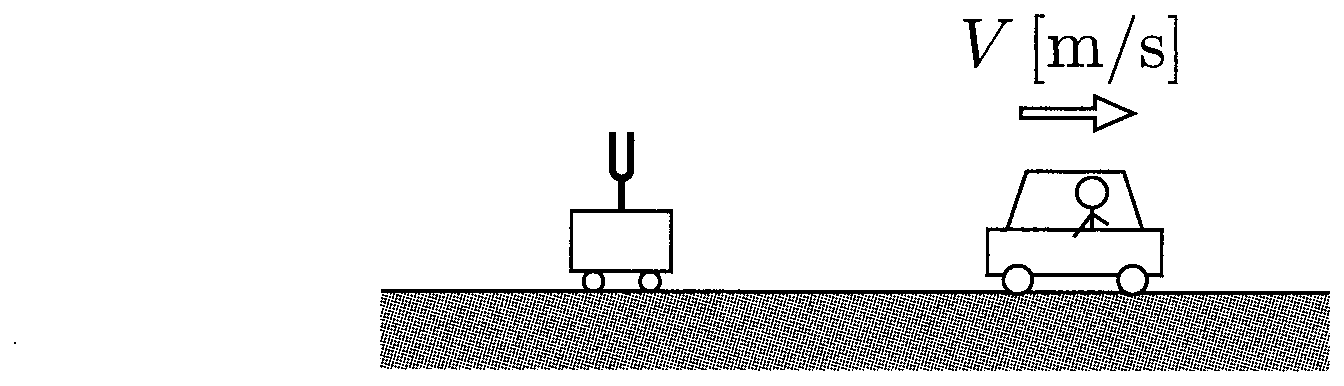
\includegraphics[keepaspectratio,width=62mm]{fig/n17_a39_z5a.png}\end{center}
       上図より，
       \[f_2=\frac{336-V}{336}\cdot1170=1086\U{Hz}\]
       である．

       救急車が動き出すと，聞こえるサイレン音の振動数が{\gtfamily 減少する}ので，これは救急車が遠ざかっていったのだと考えられる．ゆえに，救急車が走り出した向きは観測者の車の速度ベクトルとは逆向きである．その速さを$u\U{m/s}$とすると，このときの位置・速度の関係は次図のようになる．
       \begin{center}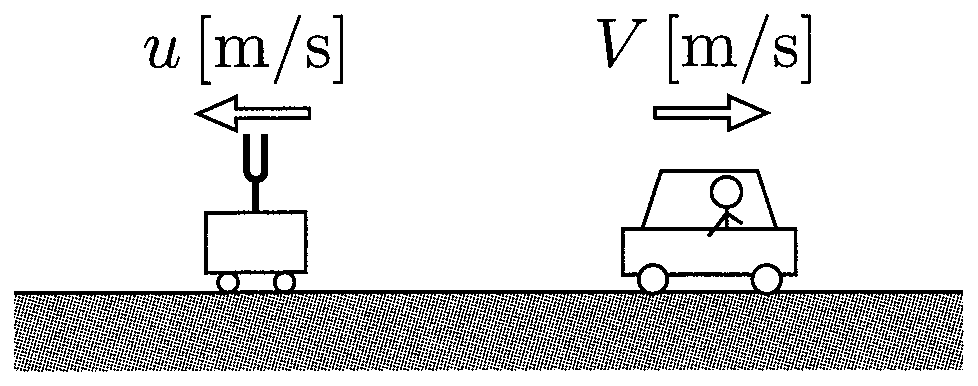
\includegraphics[keepaspectratio,width=62mm]{fig/n17_a39_z5b.png}\end{center}
       このときのドップラー効果による振動数が$1040\U{Hz}$であるから，
       \[1040=\frac{336-V}{336+u}\cdot1170\]
       が成立する．これを解いて$u\U{m/s}$を求めると，
       \[u=15\U{m/s}\]
       となる．以上より，救急車は観測者の車から遠ざかる向き（元々の進行の向きと逆向き）に速さ$15\U{m/s}$で走り始めた．\hspace*{\fill}\Ans
\end{komon}

\MonN{40}{ドップラー効果と気柱振動}\par\nopagebreak
\begin{sisin}
気柱振動とドップラー効果の融合問題で，どう考えたらよいのか見当がつかない人もいるかもしれないが，次のような手順で考えよ．開口端に着目すると，この点には波源$\mathrm{S}$の運動のためドップラー効果によって変化したある振動数の音波が到着する．ところがこの振動数の音波が実際に管の中に入り込むためには，管の中で共鳴が起こらなければならない（共鳴を起こさない振動数の音波だと，閉管に定在波が出来ないためである）．よって，管内の気柱振動が起こるためには，音源$\mathrm{S}$からやってくる音の振動数が，気柱振動の固有振動数に一致するという条件が必要であり，これを考えればよい．

(2)においては共鳴した気柱の振動が何倍振動であったかが不明である．(1)・(2)の問題文中にある「はじめて管内の気柱と共鳴した」という条件を利用して，もともとの音源の振動数$f\U{Hz}$がどの範囲にあるのかを考え，それを元に(2)は何倍振動と共鳴したのかを考えよう．閉管に発生する気柱振動の振動数は奇数倍のものしかないことに注意せよ．
\end{sisin}
\KaiHead
\begin{komon}
\ko{1} 管の開端に波源$\mathrm{S}$からやってくる音の振動数$f^\prime$は，音源移動のドップラー効果であるから，
       \[f^\prime=\frac{v}{v+u_1}f\U{Hz}\]
       である．

       また，管内に出来る気柱の基本振動の波長を$\lambda\U{m}$とすると，$\dfrac{\lambda}{4}=l$なので$\lambda=4l\U{m}$，ゆえに基本振動の振動数は$f_0=\dfrac{v}{\lambda}\U{Hz}$である．よって，気柱の$2m-1$倍振動の振動数は，
       \[(2m-1)f_0=(2m-1)\frac{v}{\lambda}\U{Hz}\]
       \begin{center}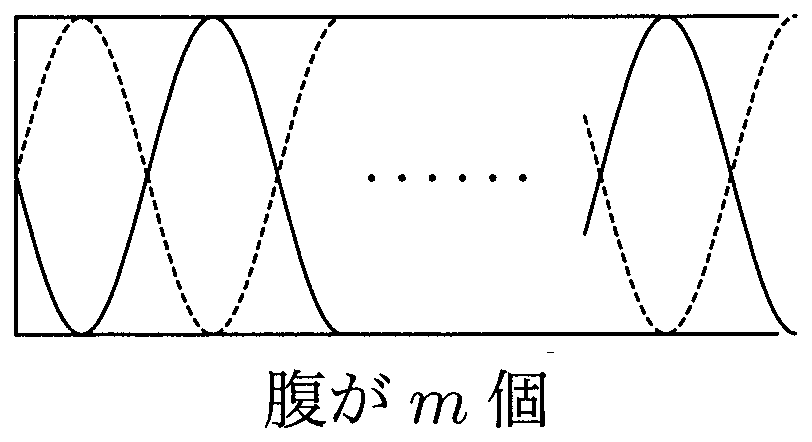
\includegraphics[keepaspectratio,width=62mm]{fig/n17_a40_z1.png}\end{center}
       であり，速さが$u_1\U{m/s}$のときにこの振動と共鳴したのであるから，
       \[(2m-1)f_0=f^\prime\]
       が成立する．これを整理すると，
       \[4fl=(2m-1)(v+u_1)\Ans\]
\ko{2} (1)において，波源$\mathrm{S}$が遠ざかると管へやってくる音波の振動数は元の$f\U{Hz}$よりも減少することになるが，$\mathrm{S}$が静止した状態からスタートして速さが$u_1\U{m/s}$となったときに初めて共鳴が起きたという条件より，$\mathrm{S}$が静止した状態において管に伝わってくる音波の振動数$f\U{Hz}$は，$2m-1$倍振動の一つ上の振動である$2m+1$倍振動の振動数$(2m+1)f_0\U{Hz}$よりも小さいということが分かる．

       (2)においては波源$\mathrm{S}$を管に近づけるが，このとき管へやってくる音波の振動数は元の$f\U{Hz}$よりも増加することになる．$(2m-1)f_0<f<(2m+1)f_0\U{Hz}$であるから，増加していって初めて共鳴が起きるのは，管の$2m+1$倍振動である振動数$(2m+1)f_0\U{Hz}$になったときである．
       \begin{center}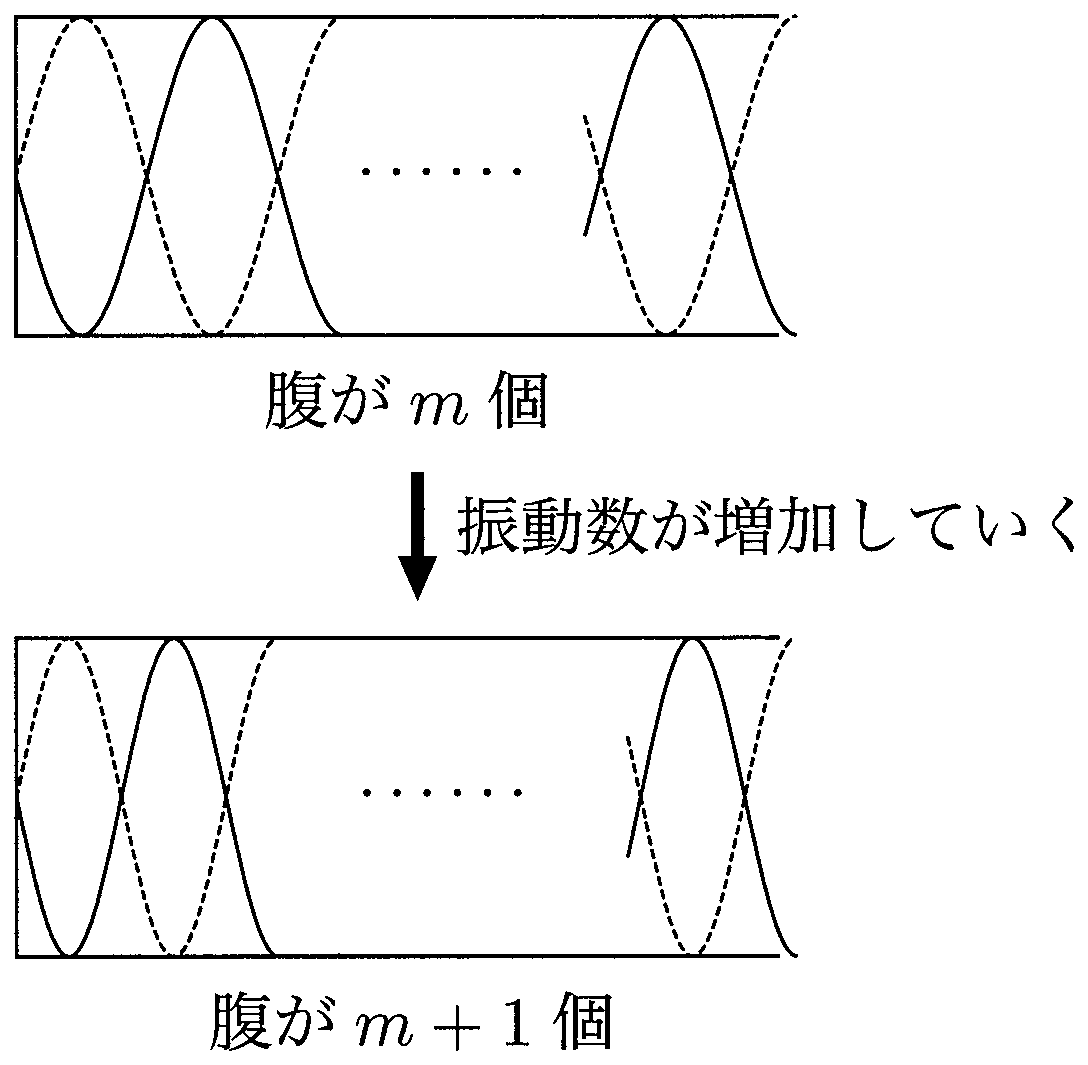
\includegraphics[keepaspectratio,width=62mm]{fig/n17_a40_z2.png}\end{center}
       よって，管の開端に波源$\mathrm{S}$からやってくる音の振動数が$(2m+1)f_0\U{Hz}$になるという式を立てると，
       \[\frac{v}{v-u_2}f=(2m+1)f_0\]
       であり，これを整理すると，
       \[4fl=(2m+1)(v-u_2)\Ans\]
\ko{3} (1)および(2)の答えに各値を代入して，
       \[4\cdot3230\cdot l=(2m-1)(336+25)\]
       \[4\cdot3230\cdot l=(2m+1)(336-13)\]
       である．これを解いて，
       \[m=9,\hspace{4mm}l=0.475\U{m}\Ans\]
\end{komon}

\MonN{41}{斜めドップラー効果と音の伝わる速さ}\par\nopagebreak
\begin{sisin}
{\gtfamily 音が伝わるのには時間がかかる}ということに注意．いつの時刻にどの場所に飛行機がいて，その点から観測者の点まで音が伝わってくるのにどれだけの時間を要するのかを，図を用いてまとめながら考えよ．
\end{sisin}
\KaiHead
\begin{komon}
\ko{1} 次図のように座標軸を取り，観測点を$\mathrm{A}$点とする．
       \begin{center}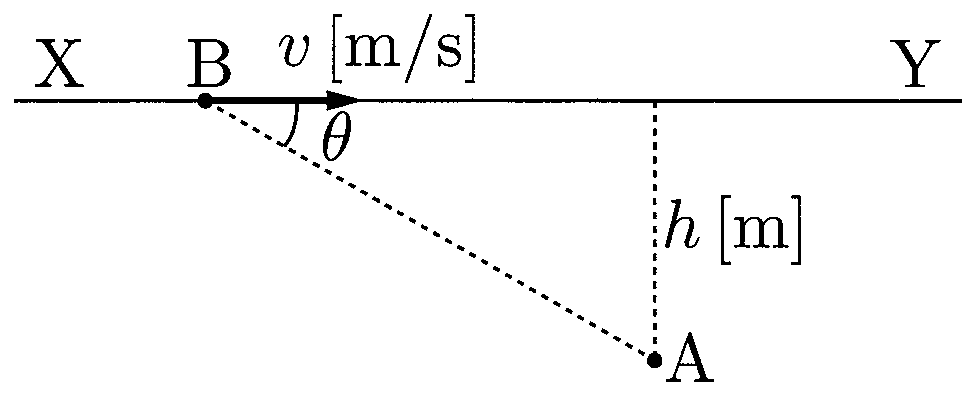
\includegraphics[keepaspectratio,width=62mm]{fig/n17_a41_z1.png}\end{center}
       飛行機が図のような角$\theta$をなす$\mathrm{B}$点において発した飛行機音は，$\mathrm{A}$点にやってきたときに
       \[f=\frac{340}{340-v\cos\theta}f_0\U{Hz}\]
       の振動数の音として聞こえる．飛行機が$\mathrm{X}$の無限遠方からやってくるときは$\theta=0^\circ$の状態に対応し，このときの振動数が
       \[f_{\max}=\lim_{\theta\to0^\circ}f=\frac{340}{340-v}f_0=3000\U{Hz}\]
       であった．また，飛行機が$\mathrm{Y}$の無限遠方に去っていくときは$\theta=180^\circ$の状態に対応し，このときの振動数が
       \[f_{\min}=\lim_{\theta\to180^\circ}f=\frac{340}{340+v}f_0=1000\U{Hz}\]
       であった．以上2式を連立させて解くと，
       \[f_0=1500\U{Hz},\hspace{4mm}v=170\U{m/s}\Ans\]
\ko{2} 飛行機の真の振動数である$f_0\U{Hz}$を観測するのは，飛行機と観測者を結ぶ速度成分が$0$となる，観測者の直上の点から音がやってきたときである．
       \begin{center}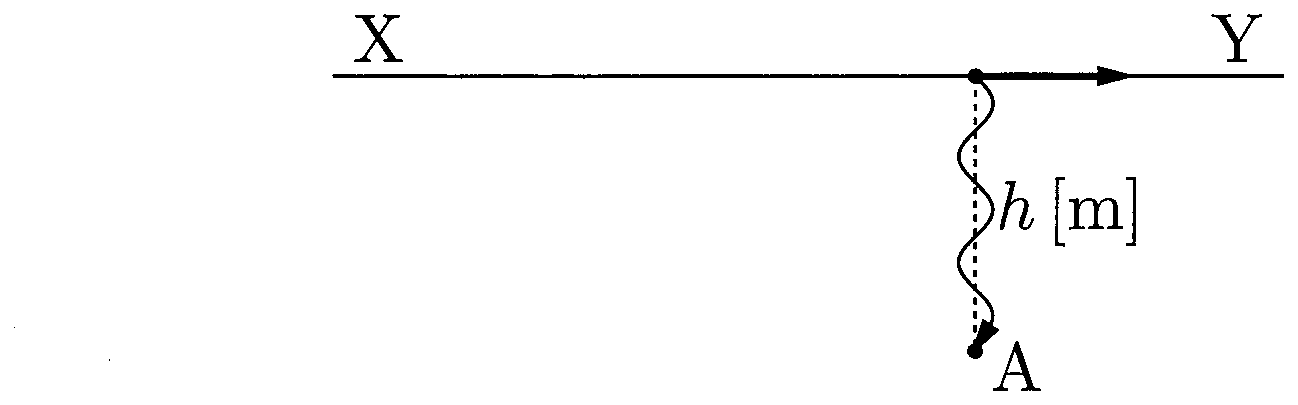
\includegraphics[keepaspectratio,width=62mm]{fig/n17_a41_z2.png}\end{center}
       飛行機が直上の点を通過した時刻は$t=0\U{s}$であり，ここで出された音が$\mathrm{A}$点に到達するまでに$3.0\U{s}$を要しているから，飛行機の高度は
       \[h=340\times3.0=1020\U{m}\Ans\]
\ko{3} 時刻$0\U{s}$において観測者が聞いた音が，角度$\varphi$をなすような次図の$\mathrm{C}$点から時刻$t_\mathrm{C}=-t_0\U{s}$に出されたものであったとする．
       \begin{center}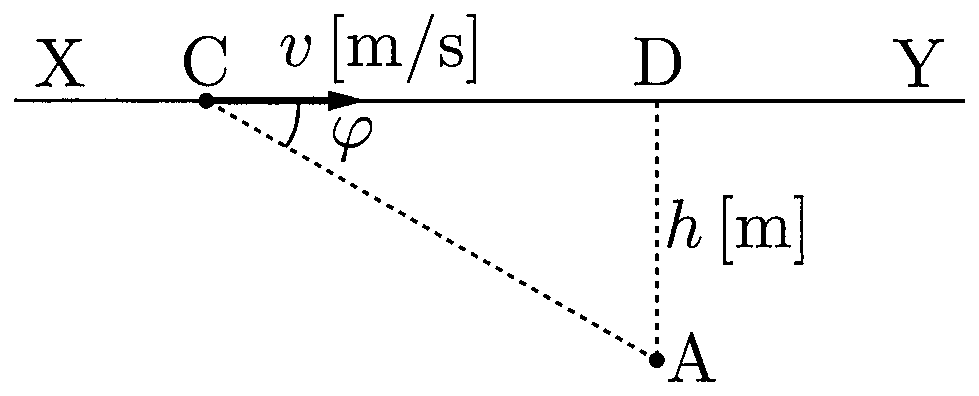
\includegraphics[keepaspectratio,width=62mm]{fig/n17_a41_z3.png}\end{center}
       このとき，
       \[\overline{\mathrm{AC}}=\frac{h}{\sin\varphi}=\frac{1020}{\sin\varphi}\U{m}\]
       であり，$\mathrm{C}$点から$\mathrm{A}$点まで音が伝わるのに$0-t_\mathrm{C}=t_0\U{s}$を要しているから，
       \[\frac{1020}{\sin\varphi}=340\cdot t_0\]
       が成立する．また，飛行機は$\mathrm{C}$点を通過したあと，時間$t_0\U{s}$後の時刻$t=0\U{s}$には$\mathrm{A}$の直上の$\mathrm{D}$点にいたのだから，
       \[\overline{\mathrm{CD}}=\frac{h}{\tan\varphi}=v\times t_0\]
       の関係が成立する．この2式を連立させて解くことにより，
       \[\cos\varphi=0.5\]
       となり，時刻$t=0\U{s}$において観測者が聞く音は，この式を満たすような角度$\varphi$の点から出された音である．求める振動数$f^\prime$は，
       \[f^\prime=\frac{340}{340-v\cos\varphi}f_0\]
       \[=\frac{340}{340-170\cdot0.5}\times1500=2000\U{Hz}\Ans\]
\end{komon}

\MonN{42}{衝撃波}\par\nopagebreak
\begin{sisin}
波源の進行速度が音速を超える場合であっても考え方は同じである．$\mathrm{P}$点で出た球面波は$\mathrm{P}$点を中心にして球面状に広がるので，$\mathrm{P}$点から出た球面波の$1\U{s}$後の半径が音速を表す．また，この間に音源は$\mathrm{Q}$点まで移動しているので，$\mathrm{PQ}$間の距離が物体の移動する速さを表す．
\end{sisin}
\KaiHead
\begin{komon}
\ko{1} 図中の大きな円は$\mathrm{P}$点から出された球面波の$1\U{s}$後の様子を表している．この間に波は$\mathrm{P}$点を中心として音速で広がっているので，この球の半径が音速$c$を表す．また，$\mathrm{PQ}$間の距離が物体の移動する速さ$v$を表しているので，この二つの関係を調べればよい．よって，
       \[\MARU{1}：c>v,\hspace{3mm}\MARU{2}：c=v,\hspace{3mm}\MARU{3}：c<v\Ans\]
\ko{2} 図の大きな円は音が$1\U{s}$間のあいだに広がることによって形成されたものであるから半径が$c$であり，$\mathrm{PQ}$間は音源が$1\U{s}$間のあいだに進んだ距離$v$を表す．よって，次図のようになる．
       \begin{center}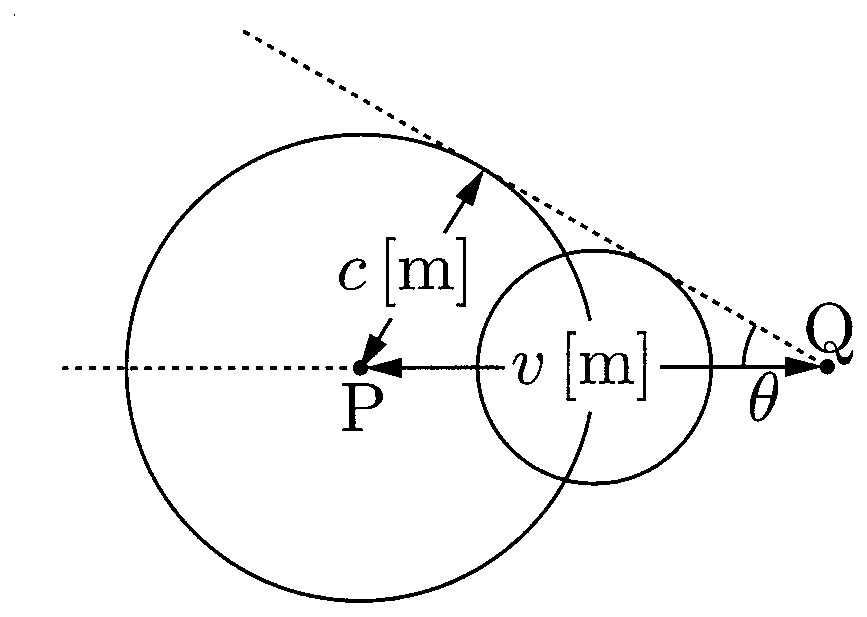
\includegraphics[keepaspectratio,width=62mm]{fig/n17_a42_z.png}\end{center}
       \[\MARU{4}：\sin\theta=\frac{c}{v}\Ans\]
\ko{3} 図(a)において$\mathrm{A}$の進行方向に伝わる波は圧縮されており，その波長は，
       \[\MARU{5}：\lambda_1=\frac{c-v}{f}\U{m}\Ans\]
       また，図(c)において$\mathrm{A}$の進行方向と逆向きに伝わる波長は伸長しており，その波長は，
       \[\MARU{6}：\lambda_2=\frac{v+c}{f}\U{m}\Ans\]
\end{komon}
\begin{bsHosoku}{参考}
この問題から分かるように，波源の速度が音速を超える場合には音は半頂角$\theta$の円錐を形成して広がっていき，波源の前方へと出ていくことはない．そのため，波源が音速を超える場合には，波源の前方ではドップラー効果は生じない．ただし，波源の後方へは音速を超えない場合と全く同様に音が発せられているので，波長変化や振動数変化は通常のドップラー効果と同様に扱うことができる．
\end{bsHosoku}

\end{multicols}
